\pdfminorversion=4
\documentclass[aspectratio=169]{beamer}

\mode<presentation>
{
  \usetheme{default}
  \usecolortheme{default}
  \usefonttheme{default}
  \setbeamertemplate{navigation symbols}{}
  \setbeamertemplate{caption}[numbered]
  \setbeamertemplate{footline}[frame number]  % or "page number"
  \setbeamercolor{frametitle}{fg=white}
  \setbeamercolor{footline}{fg=black}
} 

\usepackage[english]{babel}
\usepackage{inputenc}
\usepackage{tikz}
\usepackage{courier}
\usepackage{array}
\usepackage{bold-extra}
\usepackage{minted}
\usepackage[thicklines]{cancel}
\usepackage{fancyvrb}
\usepackage{tcolorbox}

\xdefinecolor{dianablue}{rgb}{0.18,0.24,0.31}
\xdefinecolor{darkblue}{rgb}{0.1,0.1,0.7}
\xdefinecolor{darkgreen}{rgb}{0,0.5,0}
\xdefinecolor{darkgrey}{rgb}{0.35,0.35,0.35}
\xdefinecolor{darkorange}{rgb}{0.8,0.5,0}
\xdefinecolor{darkred}{rgb}{0.7,0,0}
\definecolor{darkgreen}{rgb}{0,0.6,0}
\definecolor{mauve}{rgb}{0.58,0,0.82}

\title[2024-10-20-preCHEP-2024-codas-hep]{CoDaS-HEP and US-CMS/US-ATLAS Training}
\author{Jim Pivarski}
\institute{Princeton University -- IRIS-HEP}
\date{October 10, 2024}

\usetikzlibrary{shapes.callouts}

\usepackage{array}
\newcolumntype{L}[1]{>{\raggedright\let\newline\\\arraybackslash\hspace{0pt}}m{#1}}
\newcolumntype{C}[1]{>{\centering\let\newline\\\arraybackslash\hspace{0pt}}m{#1}}

\begin{document}

\logo{\pgfputat{\pgfxy(0.11, 7.4)}{\pgfbox[right,base]{\tikz{\filldraw[fill=dianablue, draw=none] (0 cm, 0 cm) rectangle (50 cm, 1 cm);}\mbox{\hspace{-8 cm}
\includegraphics[height=1 cm]{princeton-logo-long.png}\hspace{0.1 cm}\raisebox{0.1 cm}{
\includegraphics[height=0.8 cm]{iris-hep-logo-long.png}}\hspace{0.1 cm}}}}}

\begin{frame}
  \titlepage
\end{frame}

\logo{\pgfputat{\pgfxy(0.11, 7.4)}{\pgfbox[right,base]{\tikz{\filldraw[fill=dianablue, draw=none] (0 cm, 0 cm) rectangle (50 cm, 1 cm);}\mbox{\hspace{-8 cm}
\includegraphics[height=1 cm]{princeton-logo.png}\hspace{0.1 cm}\raisebox{0.1 cm}{
\includegraphics[height=0.8 cm]{iris-hep-logo.png}}\hspace{0.1 cm}}}}}

% Uncomment these lines for an automatically generated outline.
%\begin{frame}{Outline}
%  \tableofcontents
%\end{frame}

% START START START START START START START START START START START START START

\begin{frame}{Three of this year's HEP-computing tutorials in the U.S.}
\Large
\vspace{0.5 cm}
\begin{columns}
\column{1.08\linewidth}
\begin{itemize}\setlength{\itemsep}{0.5 cm}
\item June 20--21 (2 days): US-CMS at Princeton

\textcolor{gray}{\normalsize Alexander Held, Andrzej Novak, Elliott Kauffman, Jim Pivarski, Lindsey Gray, \\ Matthew Feickert, Nick Manganelli, Nick Smith, Oksana Shadura, Peter Elmer}

\item July 18--19 (2 days): US-ATLAS at U.\ Washington

\textcolor{gray}{\normalsize Alexander Held, Ana Peixoto, Fengping Hu, Gordon Watts, Jim Pivarski, \\ Kyungeon Choi, Lindsey Gray, Matthew Feickert, Oksana Shadura, Vangelis Kourlitis}

\item July 22--26 (5 days): CoDaS-HEP at Princeton

\textcolor{gray}{\normalsize Andres Rios-Tascon, David Lange, Henry Schreiner, Ianna Osborne, Jim Pivarski, Kilian Lieret, Louis-Guillaume Gagnon, Peter Elmer, Steve Lantz, Sudhir Malik, Tim Mattson}
\end{itemize}
\end{columns}
\end{frame}

\begin{frame}{Photos (from CoDaS-HEP)}
\vspace{0.5 cm}
\begin{columns}
\column{0.33\linewidth}
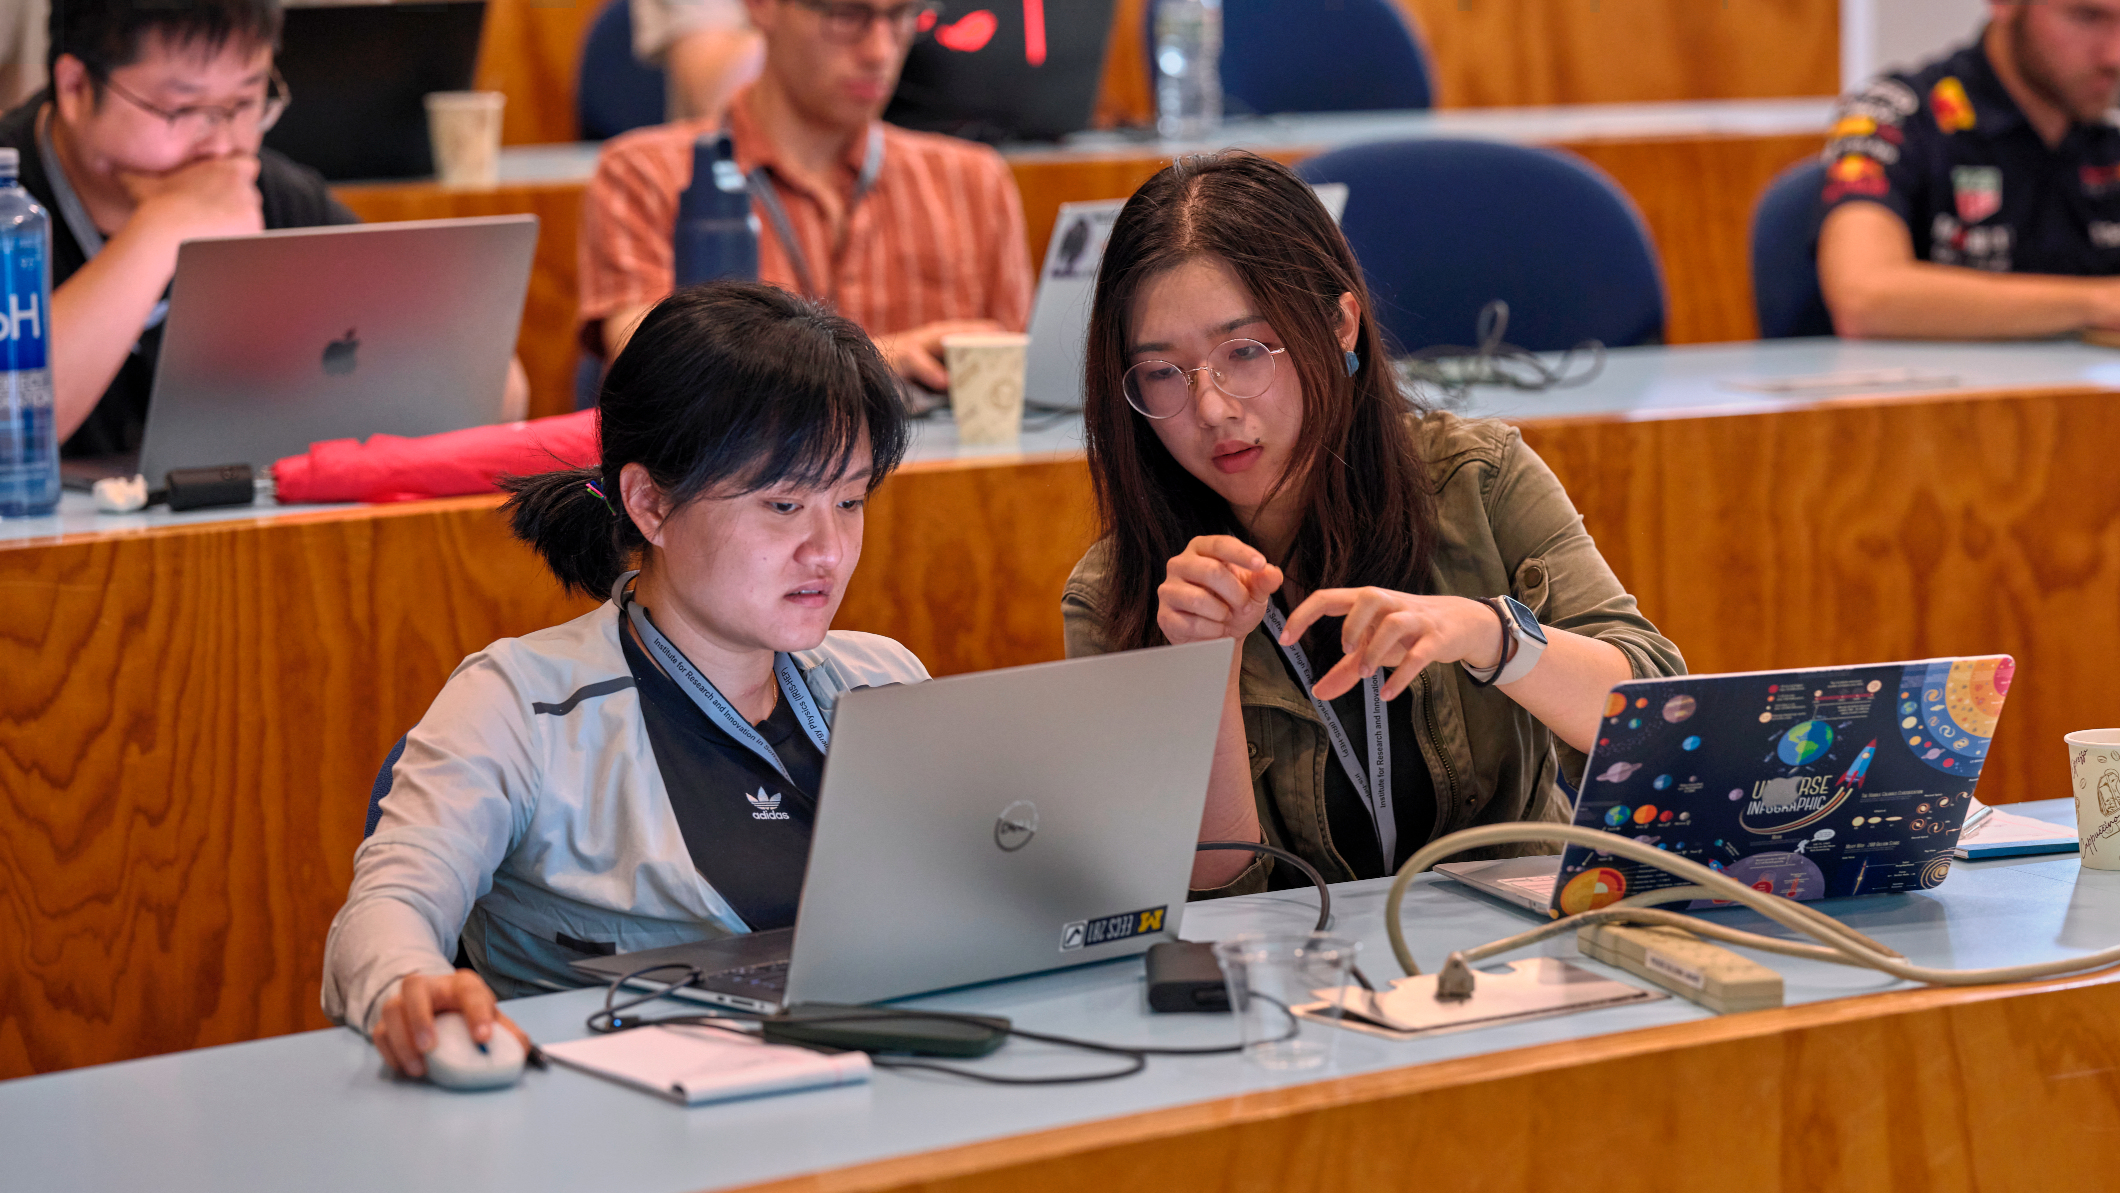
\includegraphics[width=\linewidth]{PHOTOS/DSCF2628.jpg}

\column{0.33\linewidth}
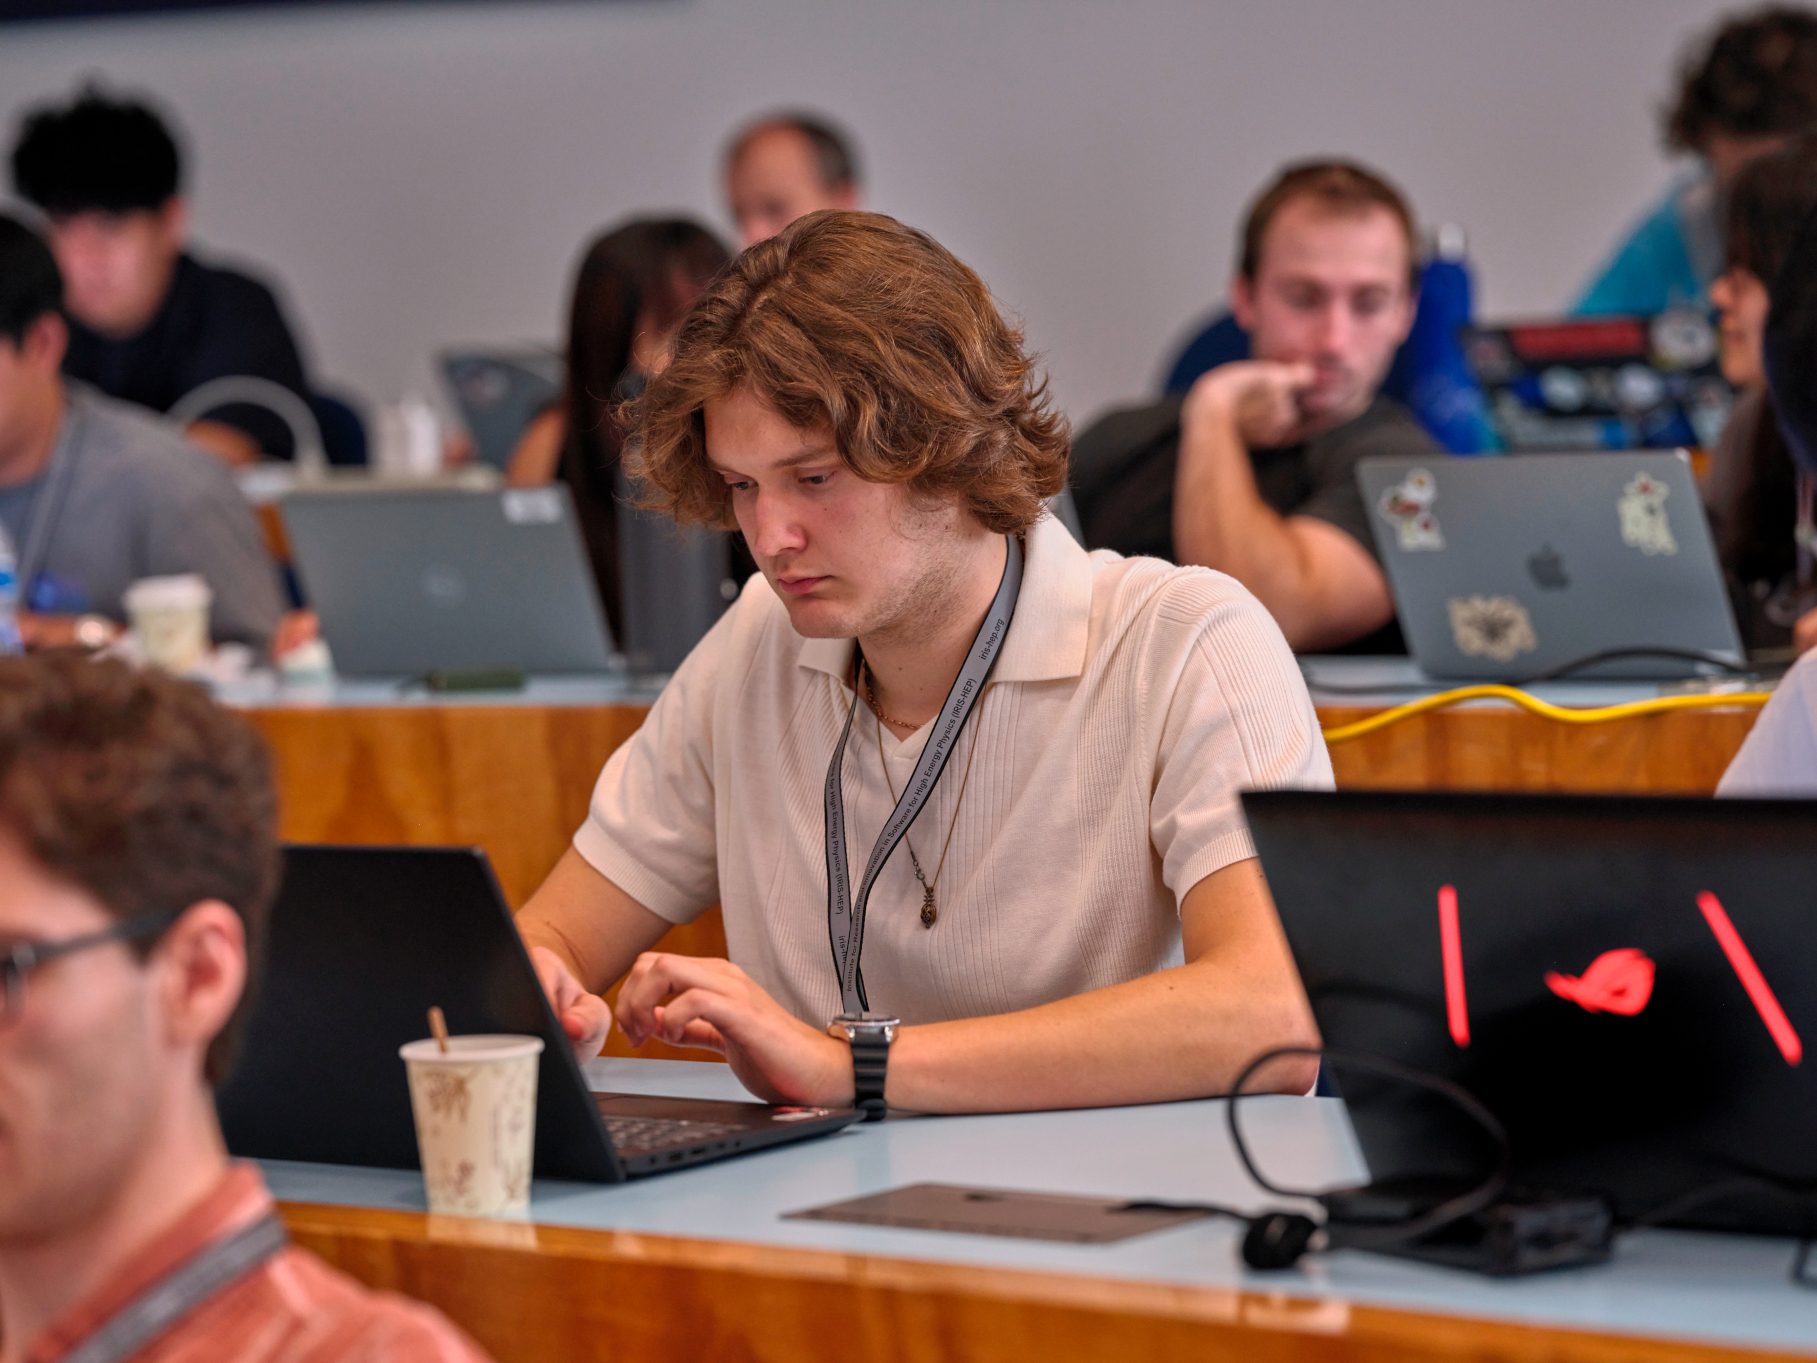
\includegraphics[width=\linewidth]{PHOTOS/DSCF2637.jpg}

\column{0.33\linewidth}
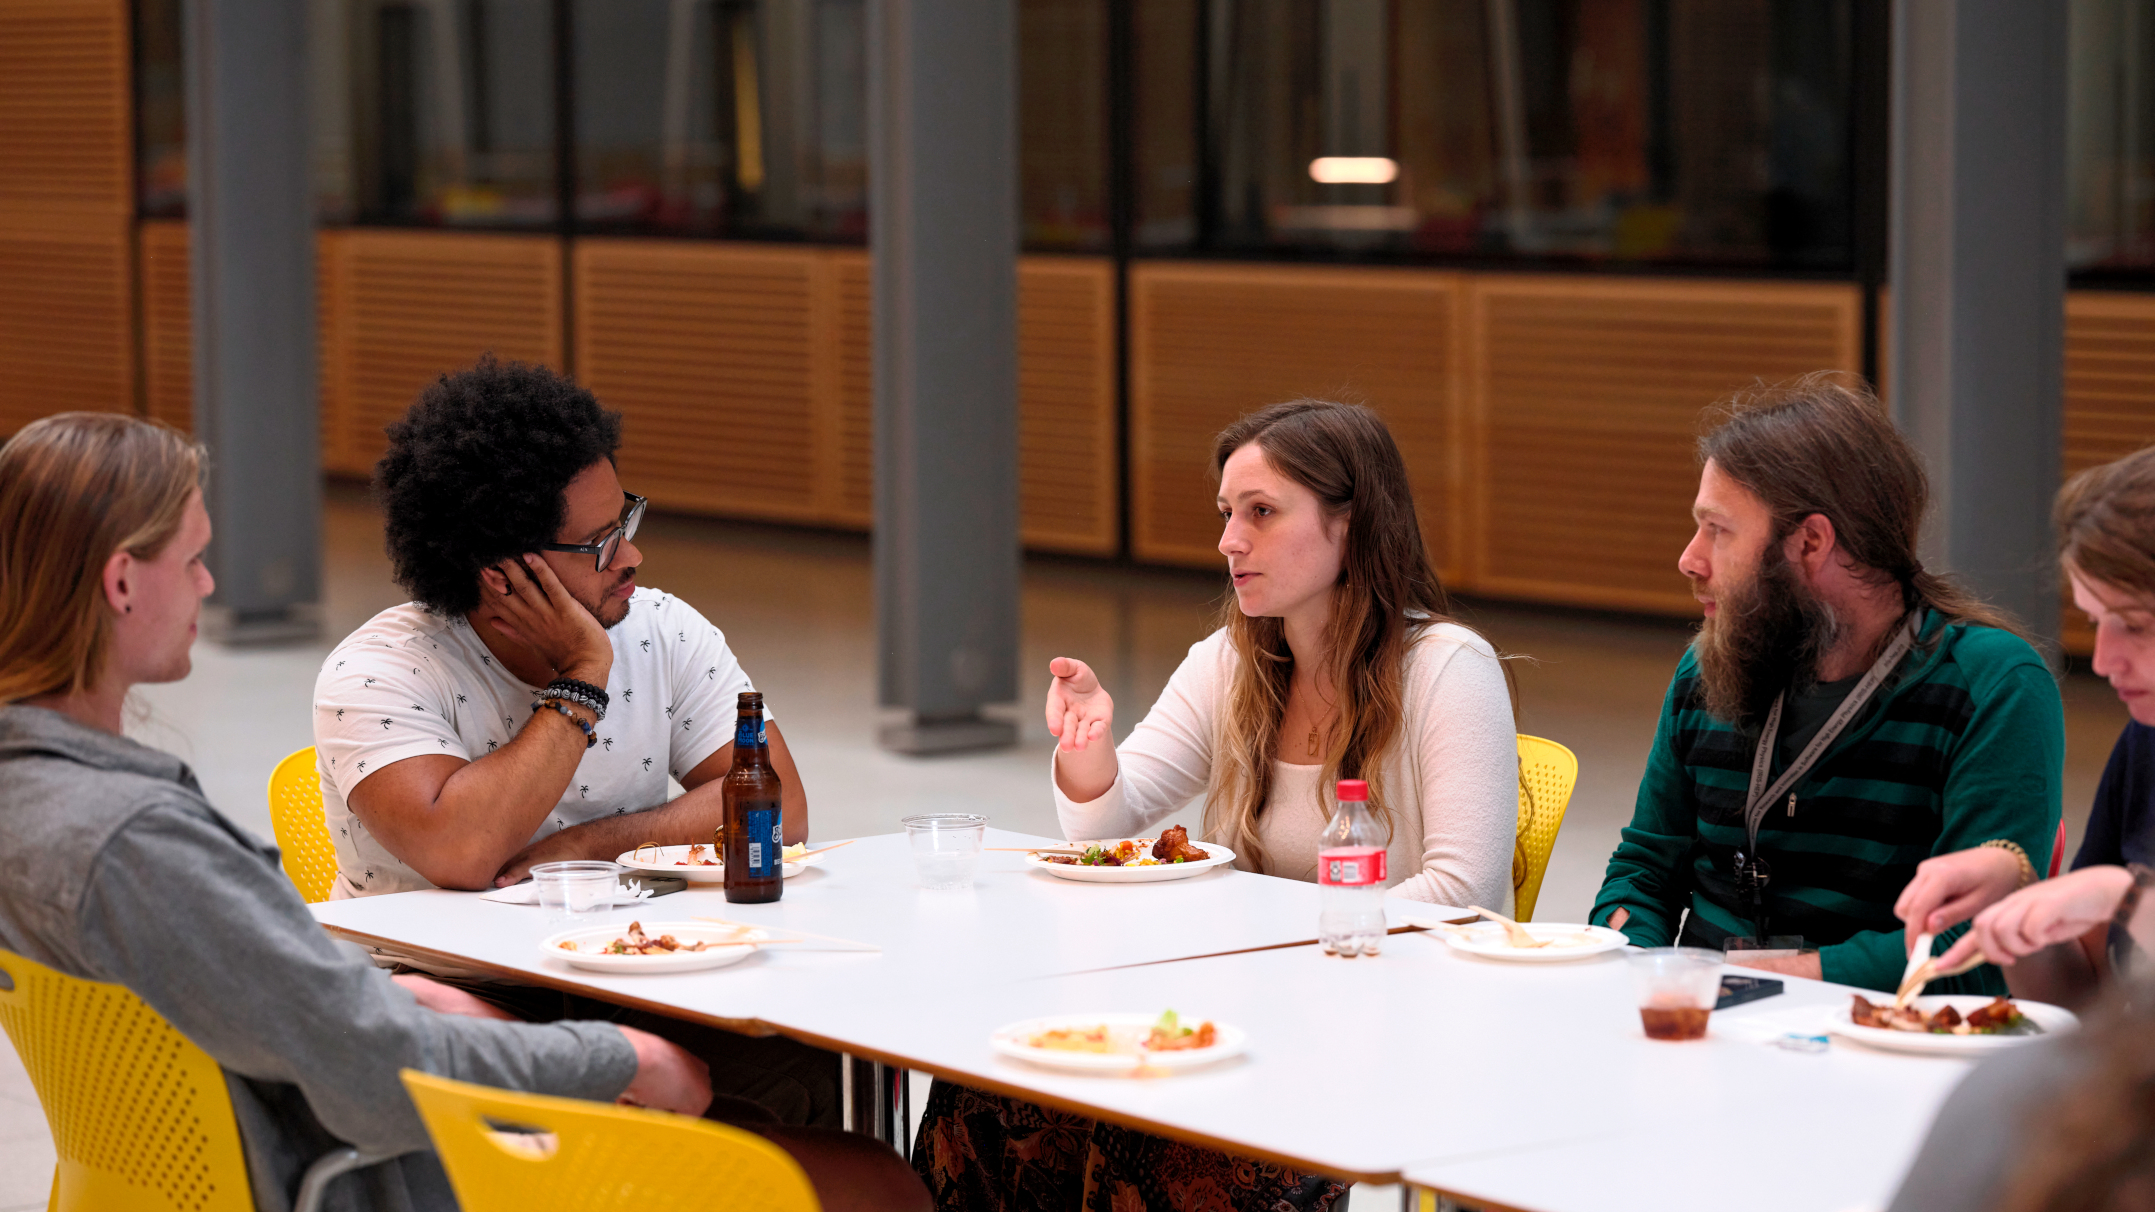
\includegraphics[width=\linewidth]{PHOTOS/DSCF2962.jpg}

%% \column{0.25\linewidth}
%% \includegraphics[width=\linewidth]{PHOTOS/DSCF3047.jpg}
\end{columns}

\begin{columns}
\column{0.33\linewidth}
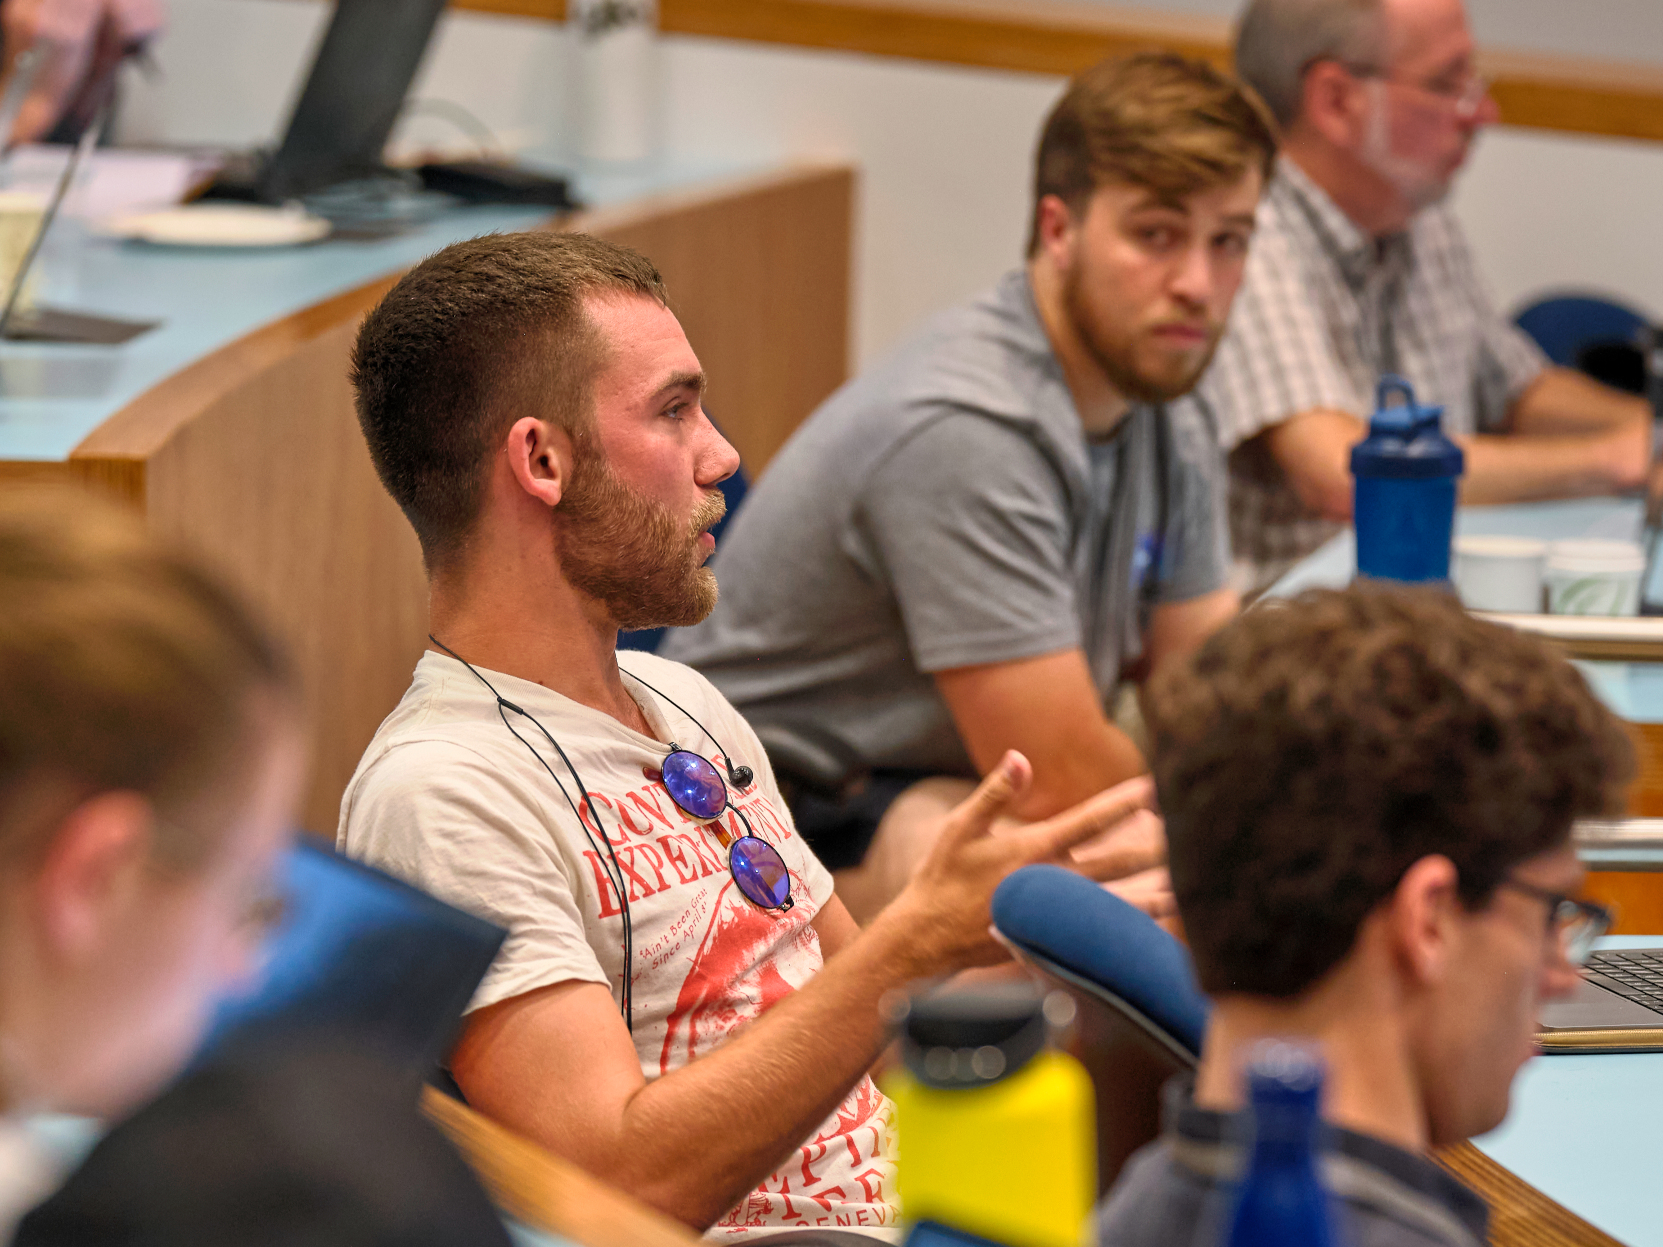
\includegraphics[width=\linewidth]{PHOTOS/DSCF2928.jpg}

\column{0.33\linewidth}
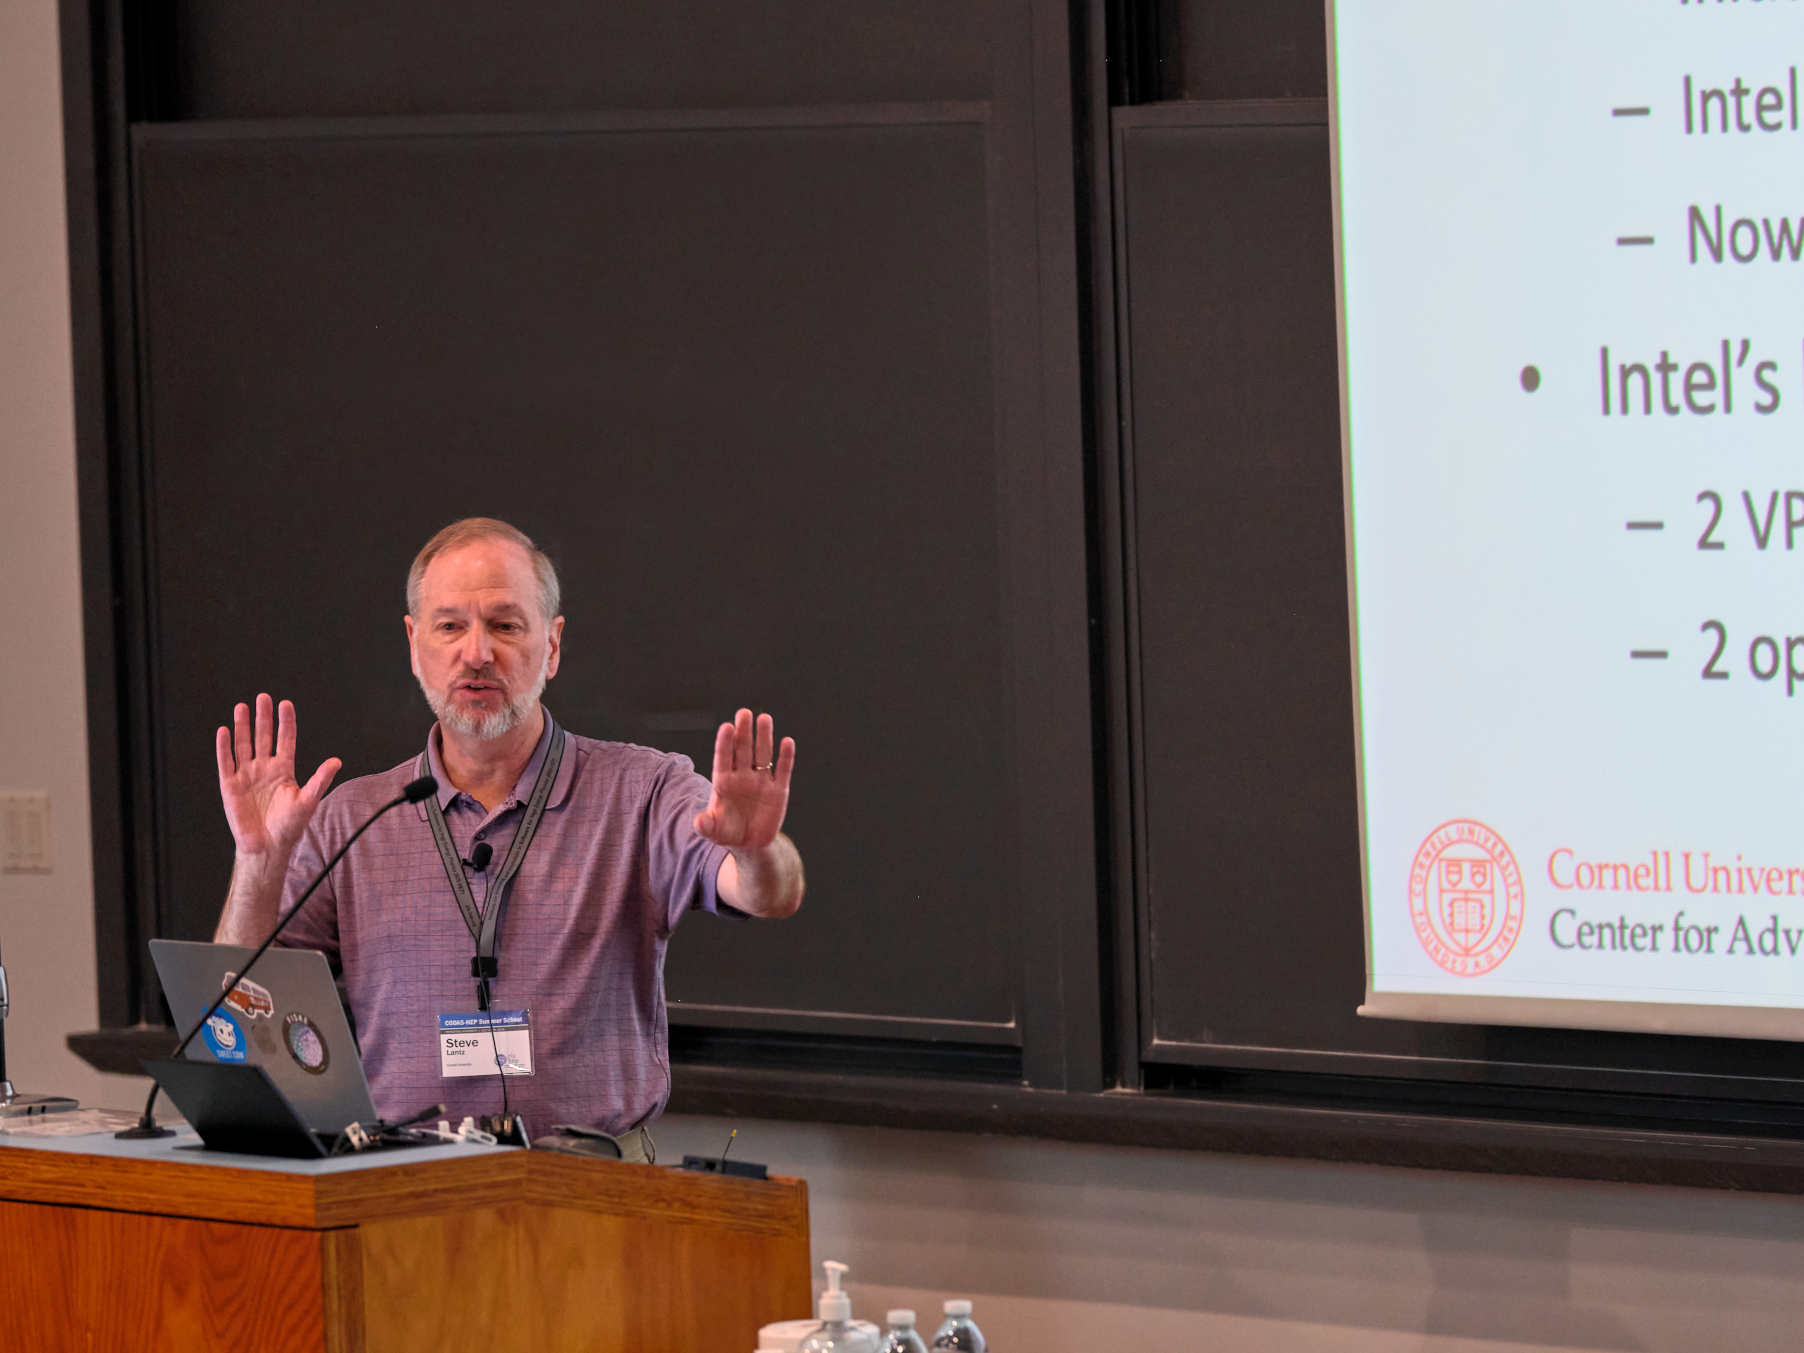
\includegraphics[width=\linewidth]{PHOTOS/DSCF2805.jpg}

\column{0.33\linewidth}
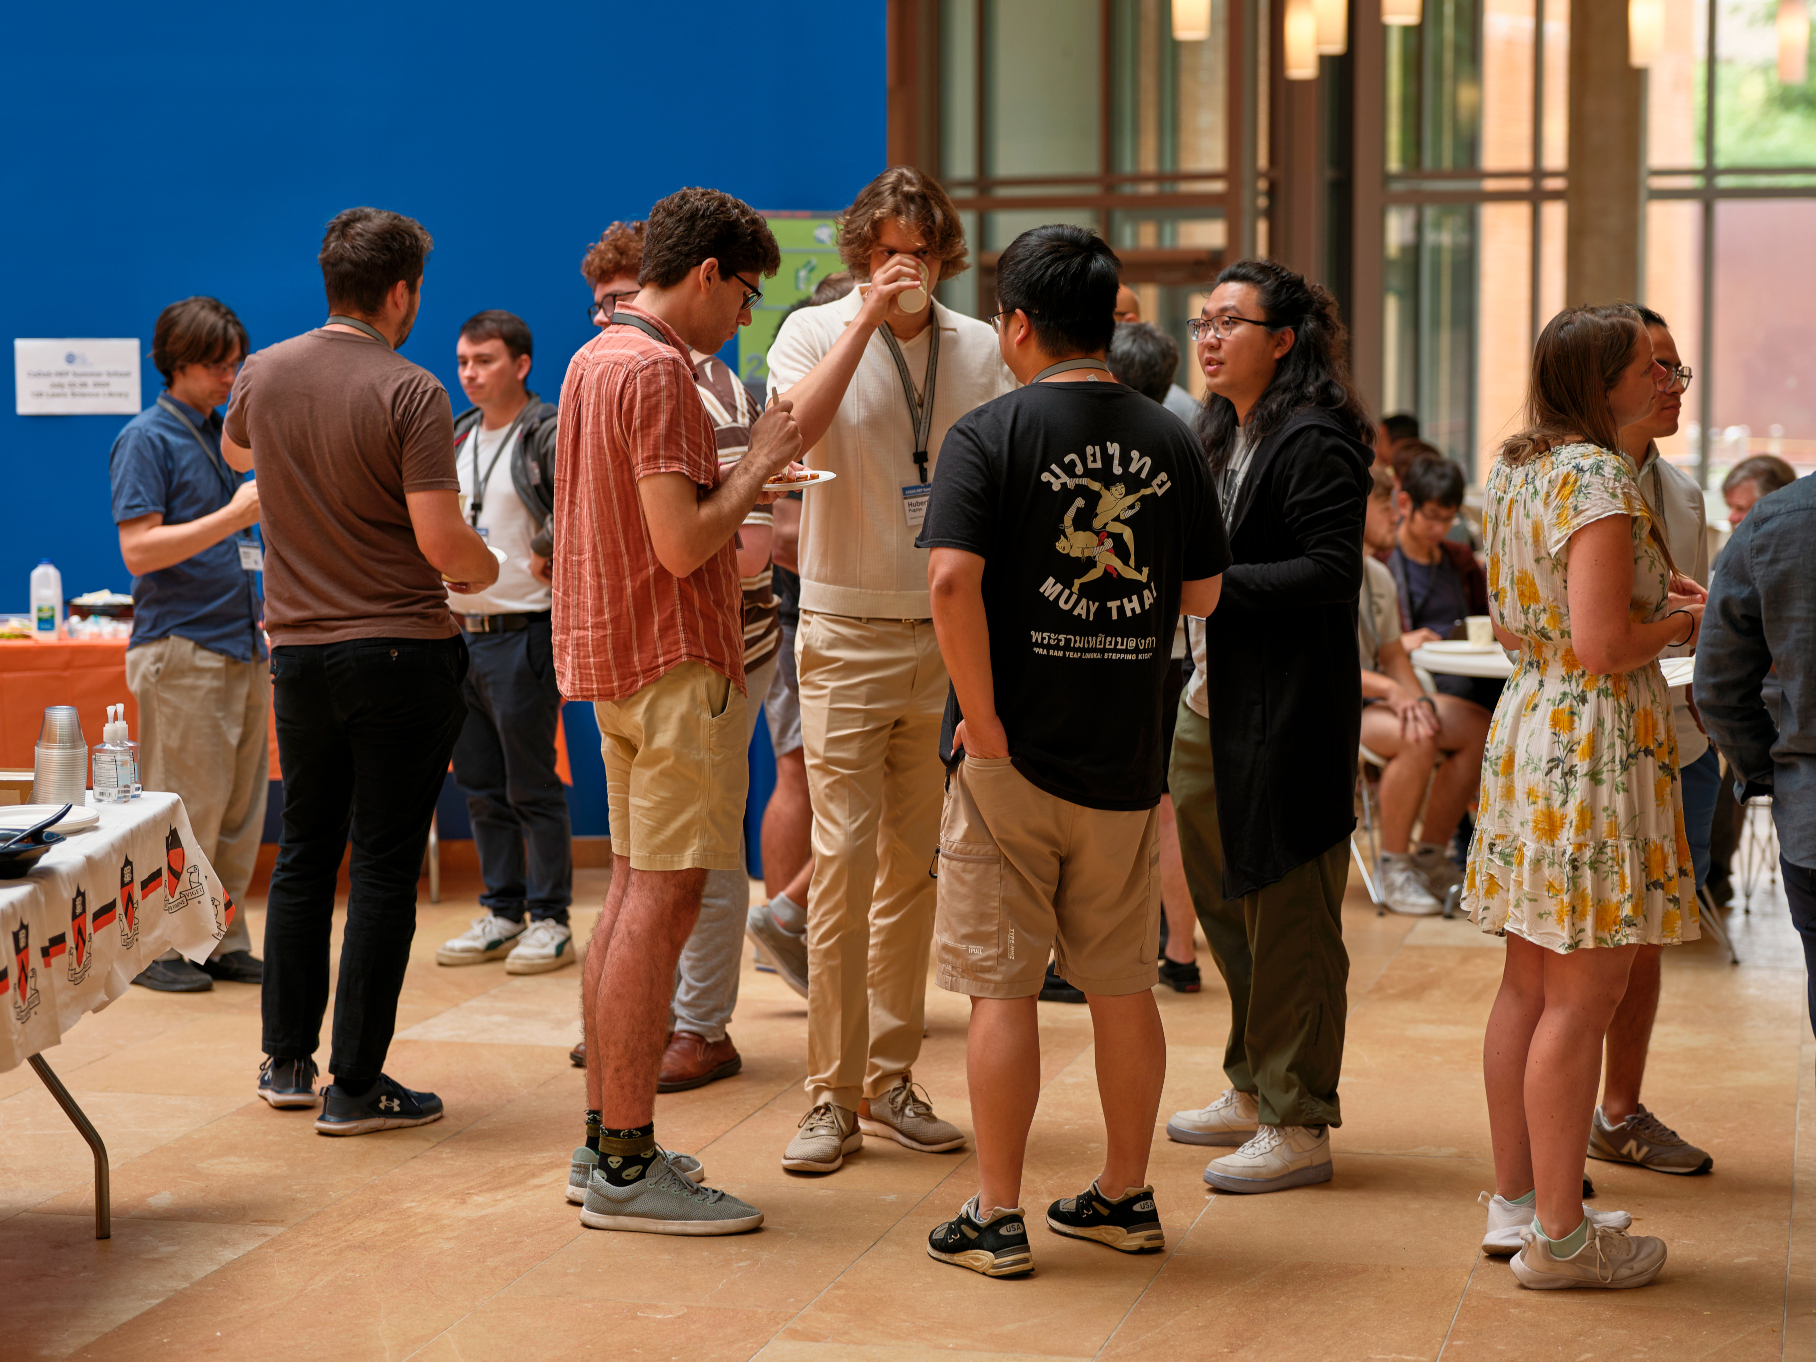
\includegraphics[width=\linewidth]{PHOTOS/DSCF2642.jpg}
\end{columns}
\end{frame}

\begin{frame}{\mbox{ }}
\LARGE
\begin{center}
\textcolor{darkblue}{Content/teaching styles/technologies}
\end{center}
\end{frame}

\begin{frame}{All three events consisted of}
\Large
\vspace{0.5 cm}
\begin{itemize}\setlength{\itemsep}{0.25 cm}
\item<1-> Lecture-style presentations (PDF, PowerPoint, Keynote)
\item<2-> Lectures mixed with small hands-on exercises (Jupyter)
\item<3-> Longer hands-on exercises: from 20 minutes to 2 hours
\item<4-> Catered breakfasts and lunches, coffee breaks
\item<5-> Social dinners and student bonding in dorms, pub crawls\ldots
\end{itemize}

\vspace{0.5 cm}
\large
\uncover<6->{Considerable sharing of teaching materials between events (including HSF-India), and from one year to the next.}

\vspace{0.25 cm}
\uncover<7->{With one exception, none of this material was from \textcolor{blue}{\url{hsf-training.org}}.}
\end{frame}

\begin{frame}{Hands-on exercises 1 (me)}
\vspace{0.25 cm}
\large
\begin{columns}
\column{0.8\linewidth}
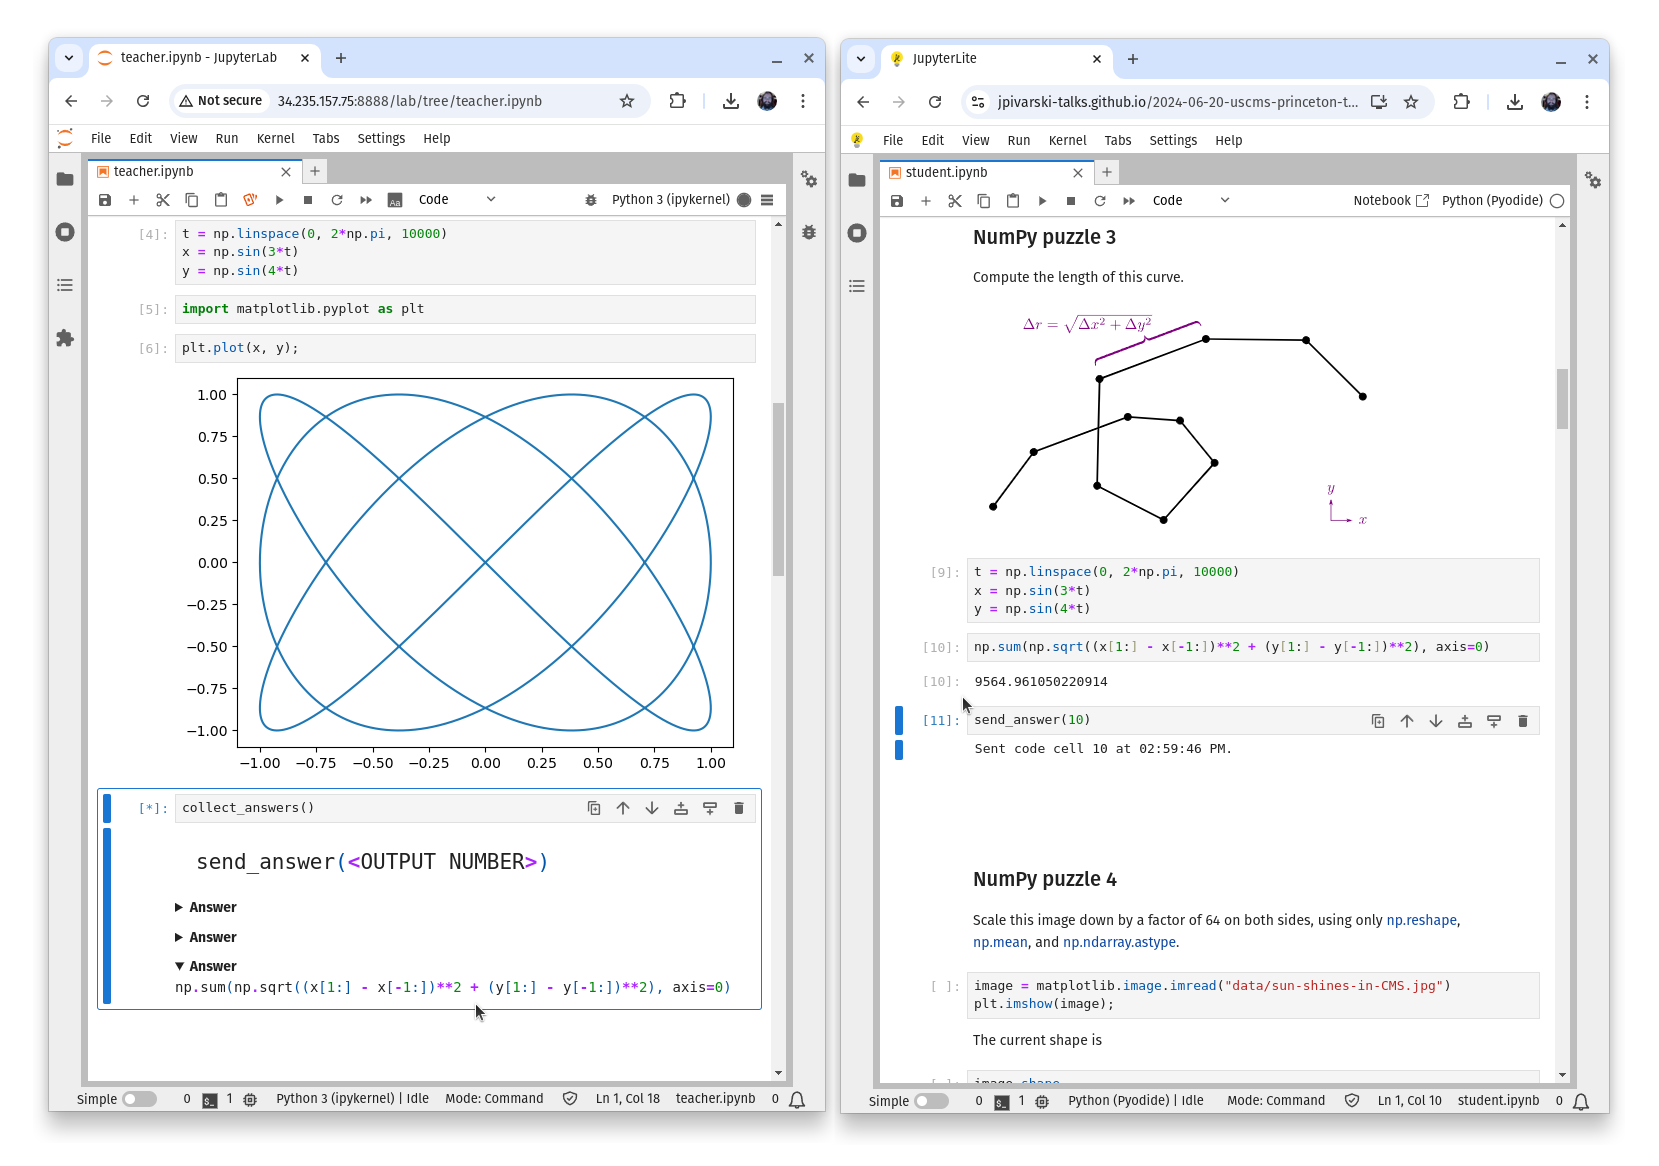
\includegraphics[width=\linewidth]{PLOTS/teacher-student-notebook-pair.png}

\column{0.3\linewidth}
\textcolor{darkorange}{\bf Columnar analysis}

\tiny
\vspace{0.2 cm}
\textcolor{blue}{\href{https://github.com/jpivarski-talks/2024-06-20-uscms-princeton-tutorial}{https://github.com/jpivarski-talks/2024-06-20-uscms-princeton-tutorial}}

\textcolor{blue}{\href{https://github.com/jpivarski-talks/2024-07-18-usatlas-seattle-tutorial}{https://github.com/jpivarski-talks/2024-07-18-usatlas-seattle-tutorial}}

\small
\vspace{0.2 cm}
\uncover<2->{Consisted almost entirely of 5--10 minute puzzles.}

\vspace{0.2 cm}
\uncover<3->{{\bf Two notebooks:} teacher.ipynb has more background, student.ipynb just sets up the problems.}

\vspace{0.2 cm}
\uncover<4->{Students \mintinline{python}{send_answer} anonymously to the teacher notebook, where we review.}

\vspace{0.2 cm}
\uncover<5->{I don't like how I had to set this up (Amazon SNS): it was too complicated.}
\end{columns}
\end{frame}

\begin{frame}{Hands-on exercises 2 (Nick Smith, Nick Manganelli, Alex Held)}
\vspace{0.25 cm}
\large
\begin{columns}
\column{0.73\linewidth}
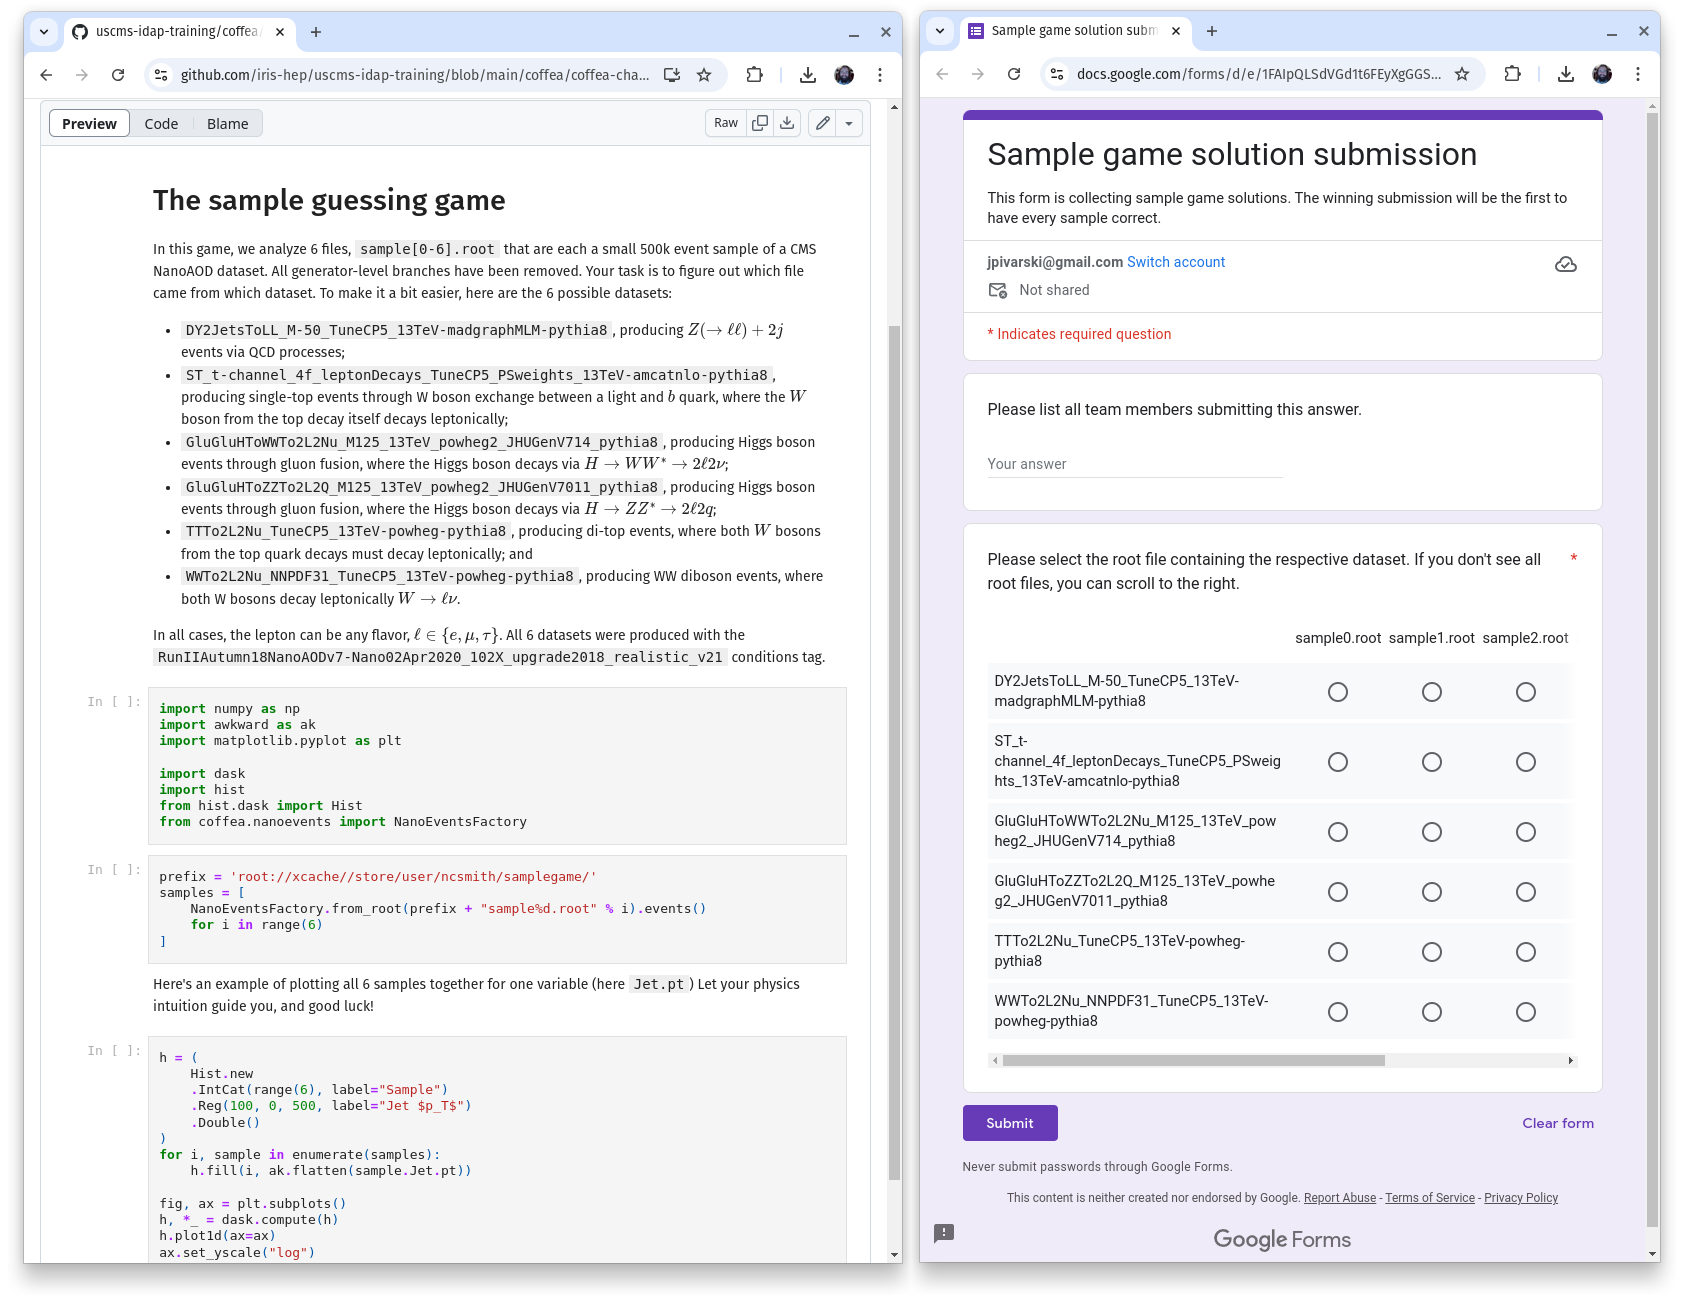
\includegraphics[width=\linewidth]{PLOTS/sample-guessing-game.png}

\column{0.3\linewidth}
\textcolor{darkorange}{\bf Sample game}

\tiny
\vspace{0.2 cm}
\textcolor{blue}{\href{https://github.com/iris-hep/uscms-idap-training/blob/main/coffea/coffea-challenge-samplegame.ipynb}{https://github.com/iris-hep/uscms-idap-training/blob/main/coffea/coffea-challenge-samplegame.ipynb}}

\scriptsize
\vspace{0.1 cm}
(from LPC HATS)

\small
\vspace{0.225 cm}
\uncover<2->{1.5 hours (+ overnight)}

\vspace{0.225 cm}
\uncover<3->{Given 6 physics samples, students use any tools necessary to figure out which was generated by which physics process.}

\vspace{0.225 cm}
\uncover<4->{Naturally, this tests both computing {\it and} physics knowledge.}

\vspace{0.225 cm}
\uncover<5->{Results are submitted in a Google Form.}
\end{columns}
\end{frame}

\begin{frame}{Hands-on exercises 3 (Kilian Lieret)}
\vspace{0.25 cm}
\large
\begin{columns}
\column{0.72\linewidth}
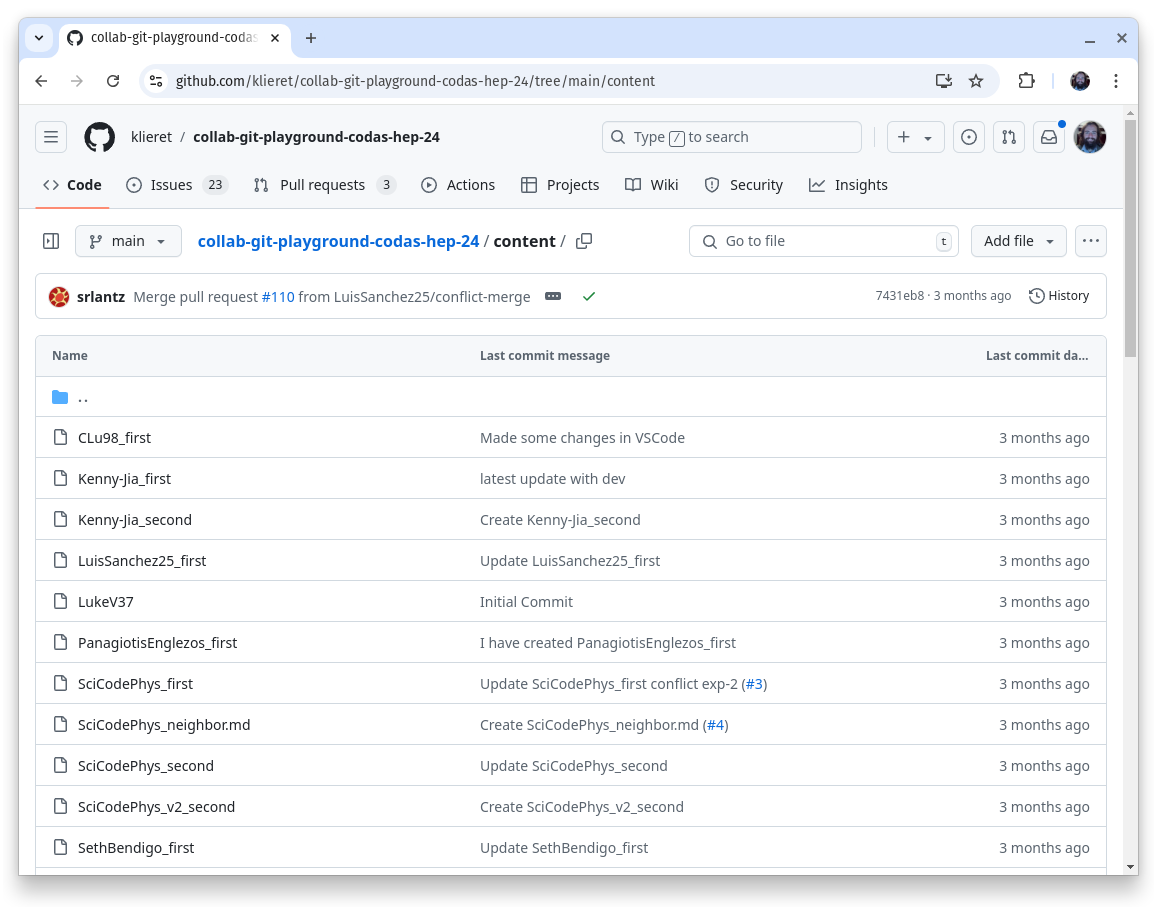
\includegraphics[width=\linewidth]{PLOTS/github-playground.png}

\column{0.3\linewidth}
\textcolor{darkorange}{\bf Git(Hub) playground}

\tiny
\vspace{0.2 cm}
\textcolor{blue}{\href{https://github.com/klieret/collab-git-playground-codas-hep-24}{https://github.com/klieret/collab-git-playground-codas-hep-24}}

\small
\vspace{0.35 cm}
\uncover<2->{1.5 hours of mixed lecture and exercises}

\vspace{0.35 cm}
\uncover<3->{Students fork, branch, open pull requests, handle merge conflicts, etc.\ in a single git repo, {\it all at the same time.}}

\vspace{0.35 cm}
\uncover<4->{The chaos that ensues is part of the learning process---this can {\it only} be done in a large group.}

\end{columns}
\end{frame}

\begin{frame}{Hands-on exercises 4 (Tim Mattson)}
\vspace{0.25 cm}
\large
\begin{columns}
\column{0.72\linewidth}
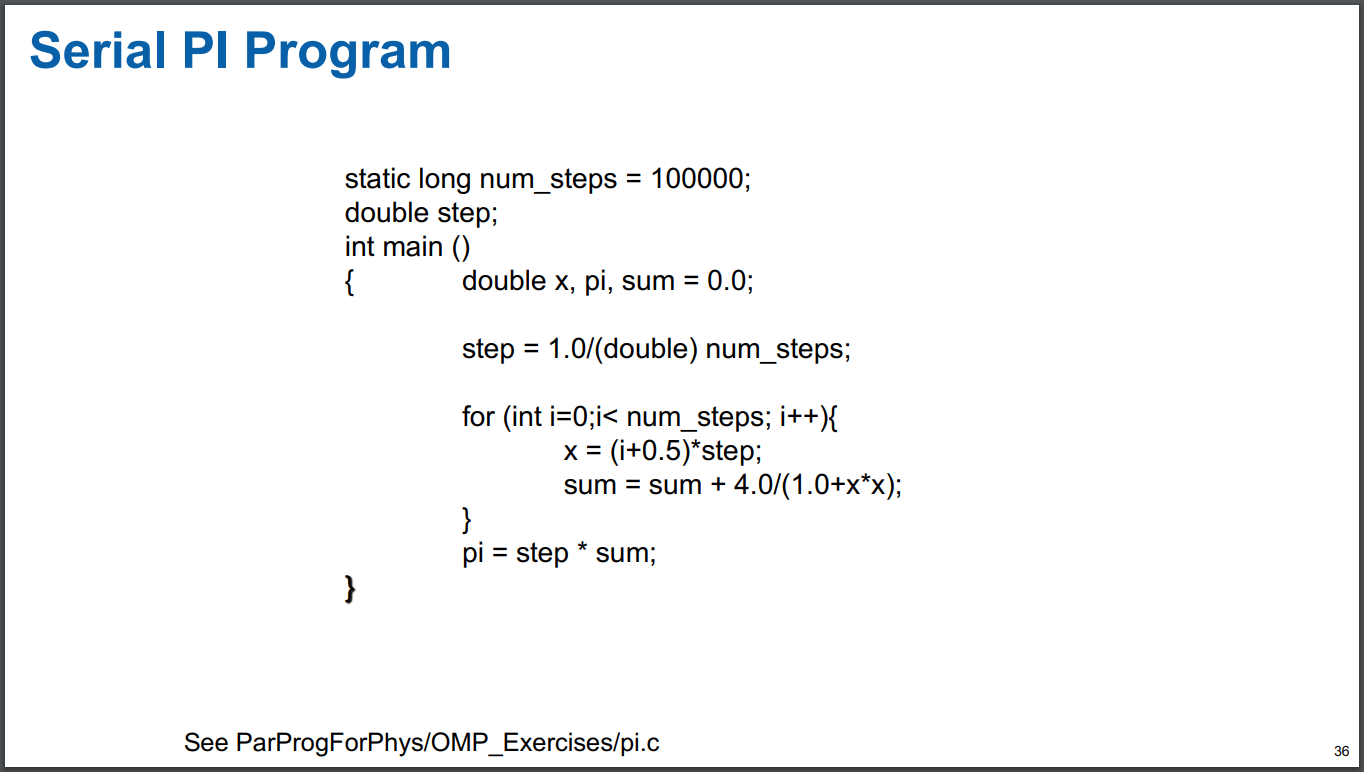
\includegraphics[width=\linewidth]{PLOTS/parallel-processing.png}

\column{0.3\linewidth}
\vspace{0.2 cm}

\textcolor{darkorange}{\bf Parallel programming}

\tiny
\vspace{0.2 cm}
\textcolor{blue}{\href{https://indico.cern.ch/event/1422680/contributions/5983265/attachments/2900081/5085486/intro_par_prog_with_Openmp.pdf}{https://indico.cern.ch/event/1422680/ \\
%
contributions/5983265/attachments/2900081/
%
5085486/intro\_par\_prog\_with\_Openmp.pdf}}

\small
\vspace{0.2 cm}
\uncover<2->{1/2 hour per problem}

\vspace{0.2 cm}
\uncover<3->{Students copy serial programs, compile them, and parallelize them.}

\vspace{0.2 cm}
\uncover<4->{Making students type whole programs manually is a good learning experience!}

\vspace{0.2 cm}
\uncover<5->{Students who can't install an OpenMP-enabled compiler on their laptop can use JupyterLab's text editor and terminal.}

\end{columns}
\end{frame}

\begin{frame}{Hands-on exercises 5 (Yana Osborne and me)}
\vspace{0.25 cm}
\large
\begin{columns}
\column{0.73\linewidth}
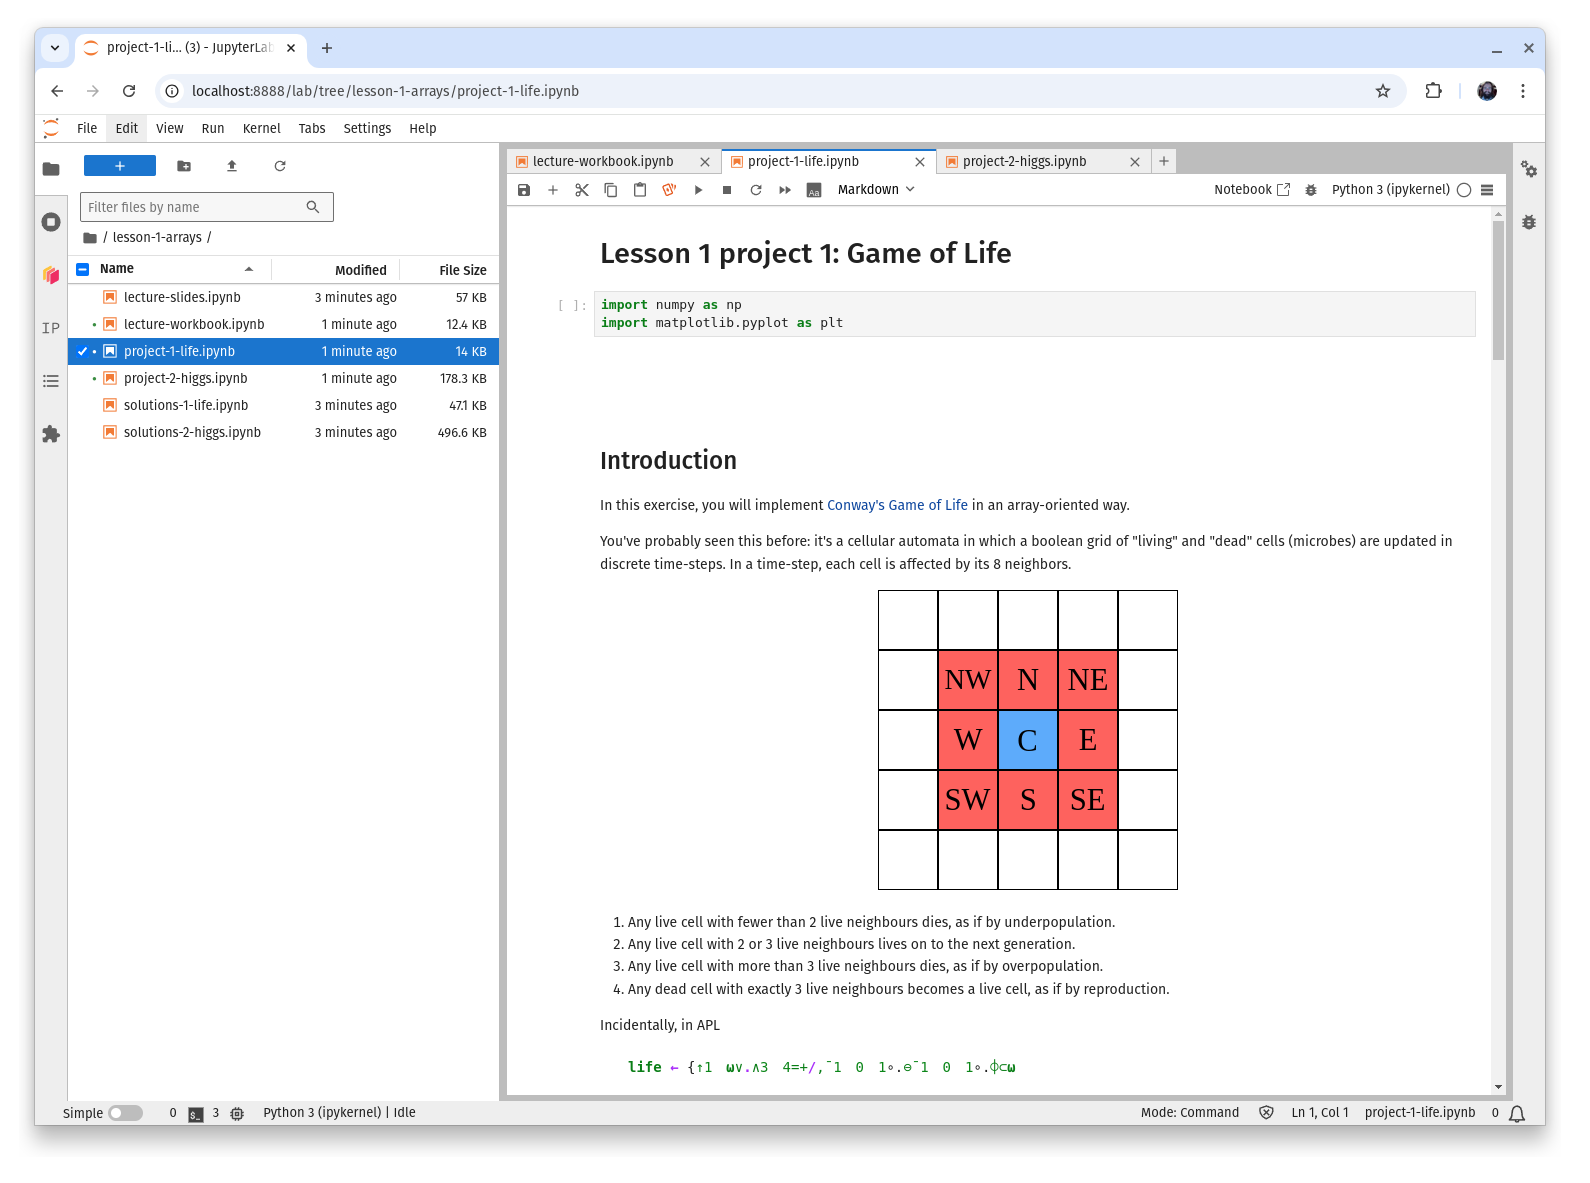
\includegraphics[width=\linewidth]{PLOTS/long-form-problem-sets.png}

\column{0.3\linewidth}
\textcolor{darkorange}{\bf Columnar analysis}

\tiny
\vspace{0.2 cm}
\textcolor{blue}{\href{https://github.com/ianna/2024-07-24-codas-hep-columnar-data-analysis}{https://github.com/ianna/2024-07-24-codas-hep-columnar-data-analysis}}

\small
\vspace{0.25 cm}
\uncover<2->{Each lesson has lecture with short problems in slides (jupyterlab-deck) and a workbook (Jupyter), like the teacher/student pair of notebooks, but also has two long (1/2 hour) problems.}

\small
\vspace{0.25 cm}
\uncover<3->{Slides + workbook is done together, but long problems are on their own/in groups.}

\small
\vspace{0.25 cm}
\uncover<4->{Since there's a choice of problems, it's hard to present solutions.}
\end{columns}
\end{frame}

\begin{frame}{Hands-on exercises 6 (me)}
\vspace{0.25 cm}
\large
\begin{columns}
\column{0.72\linewidth}
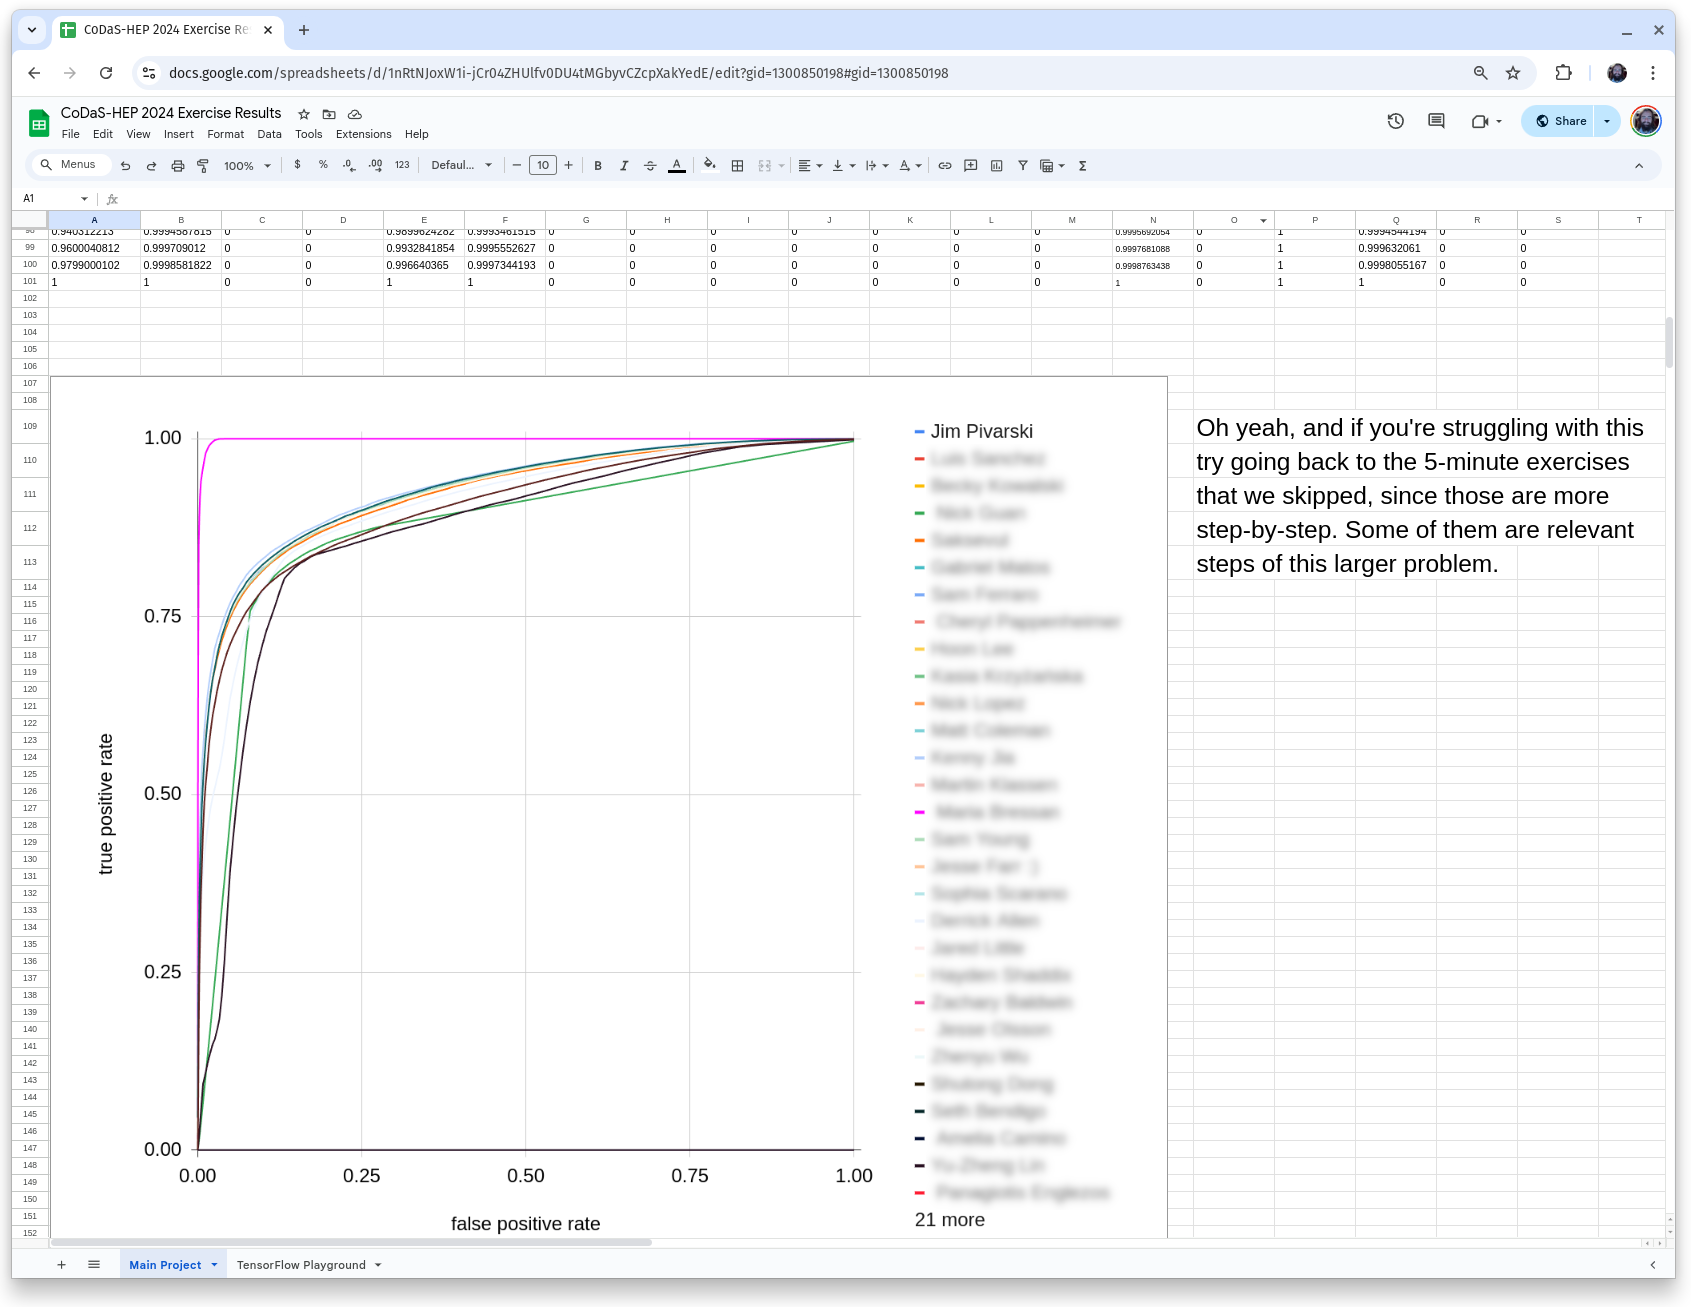
\includegraphics[width=\linewidth]{PLOTS/ml-results-in-google-sheet.png}

\column{0.3\linewidth}
\textcolor{darkorange}{\bf Machine learning}

\tiny
\vspace{0.2 cm}
\textcolor{blue}{\href{https://github.com/jpivarski-talks/2024-07-24-codas-hep-ml}{https://github.com/jpivarski-talks/2024-07-24-codas-hep-ml}}

\small
\vspace{0.25 cm}
\uncover<2->{After a lecture with small problems, students had to build a neural network from scratch in 2 hours (data and problem given).}

\small
\vspace{0.25 cm}
\uncover<3->{Results were collected in a shared Google spreadsheet: they pasted ROC curve results into a column and all results were plotted.}

\small
\vspace{0.25 cm}
\uncover<4->{(Much easier to set up than \mintinline{python}{send_answer}.)}
\end{columns}
\end{frame}

\begin{frame}{General comments/conclusions}
\large
\vspace{0.5 cm}
\begin{itemize}\setlength{\itemsep}{0.45 cm}
\item<1-> We know what we want to teach; it's easy to write talks/lectures on these topics but hard to create hands-on problems at the right level: we informally reuse them by copy-paste-and-edit.
\item<2-> \textcolor{blue}{\url{hsf-training.org}} would be more useful to us as a repository of problem sets that we can mix into our lessons, rather than full lessons.
\item<3-> We also want to feed student solutions back into the main lecture, to discuss them, and we have been trying different technologies to do that.
\begin{itemize}
\item It's easier with an off-the-shelf product, like Google Sheets, Forms, and GitHub.
\end{itemize}
\item<4-> There are reasons to have both
\begin{itemize}
\item short problems to keep students engaged in a lecture, ``on rails'' to keep them short,
\item long problems to simulate real problem-solving, ``open world'' for realism.
\end{itemize}

\end{itemize}
\end{frame}

\begin{frame}{\mbox{ }}
\LARGE
\begin{center}
\textcolor{darkblue}{Getting software to students}
\end{center}
\end{frame}

\begin{frame}{This is a surprisingly hard problem}
\vspace{0.3 cm}
\begin{columns}
\column{1.1\linewidth}\setlength{\extrarowheight}{-0.15 cm}
\begin{tabular}{p{0.3\linewidth} p{0.35\linewidth} C{0.14\linewidth} C{0.12\linewidth}}
{\bf Method} & {\bf Failure modes} & {\bf P(works for everyone)} & {\bf Reusable afterward} \\\hline
\uncover<1->{Have students install everything on their own laptops; venv, conda-forge, Docker} & \uncover<1->{Windows; not having the software to install the software; mystery errors we can't spend time to solve} & \uncover<1->{\vspace{-0.4 cm}$1 - 0.9^N$} & \uncover<1->{\vspace{-0.4 cm}yes} \\
\uncover<2->{Public cloud-based Binder (\textcolor{blue}{\href{mybinder.org}{mybinder.org}})} & \uncover<2->{Stuck loading image; crashes without persistence} & \uncover<2->{\vspace{-0.4 cm}$0.8$} & \uncover<2->{\vspace{-0.4 cm}yes} \\
\uncover<3->{GitHub Codespaces} & \uncover<3->{Big images; boots in VSCode, not Jupyter (unless configured to)} & \uncover<3->{\vspace{-0.4 cm}$0.95$} & \uncover<3->{\vspace{-0.4 cm}yes} \\
\uncover<4->{Google Colab (with GPUs!)} & \uncover<4->{Persistence; not Jupyter (old fork)} & \uncover<4->{\vspace{-0.4 cm}$0.95$} & \uncover<4->{\vspace{-0.4 cm}yes} \\
\uncover<5->{CERN Swan} & \uncover<5->{CERN accounts} & \uncover<5->{\vspace{-0.4 cm}$1 - 0.8^N$} & \uncover<5->{\vspace{-0.4 cm}yes} \\
\uncover<6->{Paid cloud solution} & \uncover<6->{Authentication} & \uncover<6->{\vspace{-0.4 cm}$0.95$} & \uncover<6->{\textcolor{red}{\vspace{-0.4 cm}no}} \\
\uncover<7->{In-browser JupyterLite} & \uncover<7->{Not all packages can be used} & \uncover<7->{\vspace{-0.4 cm}\textcolor{red}{$1$}} & \uncover<7->{\vspace{-0.4 cm}yes} \\
\raggedright \uncover<8->{Self-hosted JupyterHub} & \uncover<8->{Authentication; big images; GPUs} & \uncover<8->{\vspace{-0.4 cm}$0.9$} & \uncover<8->{\vspace{-0.4 cm}maybe} \\
\end{tabular}
\end{columns}
\end{frame}

\begin{frame}{\mbox{ }}
\large
\vspace{1 cm}
More on ``Self-hosted JupyterHub/BinderHub'' in David Lange's HSF-India talk.
\end{frame}

\begin{frame}{\mbox{ }}
\LARGE
\begin{center}
\textcolor{darkblue}{Feedback from students}
\end{center}
\end{frame}

\begin{frame}{Student surveys}
\Large
\vspace{0.5 cm}
CoDaS-HEP was held in 2017, 2018, 2019, 2022, 2023, and 2024.

\vspace{0.5 cm}
\uncover<2->{I could find survey results from all but 2019.}

\vspace{0.5 cm}
\uncover<3->{Survey consists of quantitative rankings and qualitative requests for comments, some general and some per-teacher/session.}

\vspace{0.5 cm}
\uncover<4->{Per-teacher questions are useful for improving the program, but we'll only look at general questions here.}
\end{frame}

\begin{frame}{General quantitative questions}
\large
\vspace{0.2 cm}
\begin{columns}
\column{0.7\linewidth}
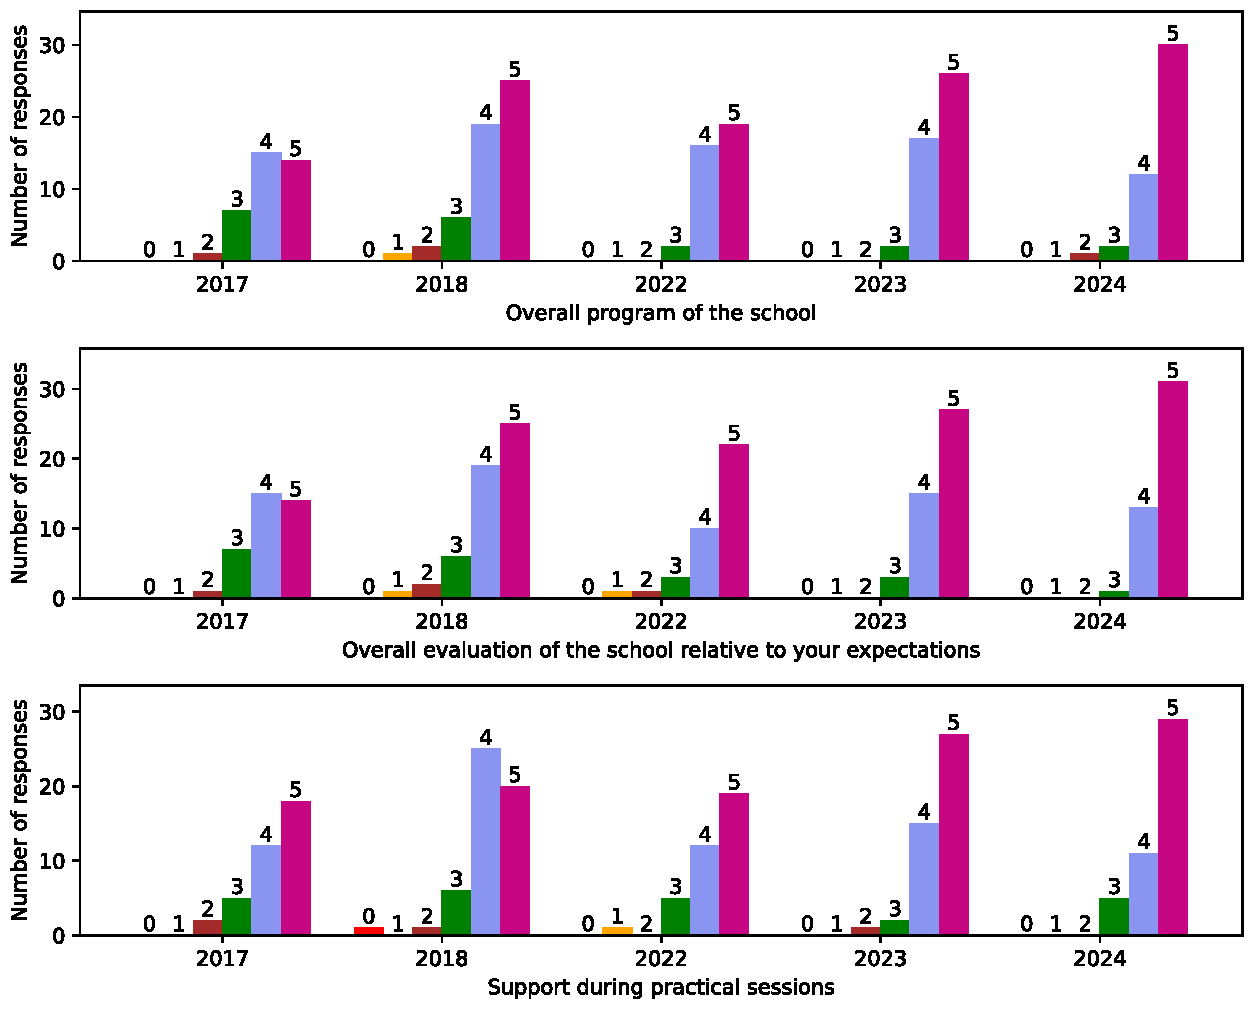
\includegraphics[width=\linewidth]{PLOTS/evaluations_by_year.pdf}

\column{0.3\linewidth}
Mostly unchanging, mostly positive.

\vspace{1 cm}
\uncover<2->{They reflect well on us, but aren't useful for making decisions or changes.}
\end{columns}
\end{frame}

\begin{frame}{Analyzing qualitative data: the free-form comment boxes}
\vspace{0.5 cm}
The students made a lot of good suggestions, but
\begin{itemize}
\item what were the most common suggestions?
\item how can I show them without explicit quotes? (We didn't say they'd be public.)
\end{itemize}

\vspace{1 cm}
\begin{uncoverenv}<2->
I can summarize them for you, but
\begin{itemize}
\item my diligence might not be constant: I might weigh early comments more than later ones (there's a lot of text to read),
\item some of the comments are about me: how can I convince you/myself that I've summarized them fairly?
\end{itemize}
\end{uncoverenv}
\end{frame}

\begin{frame}[fragile]{Trying a new thing: CharGPT for semantic clustering}
\tiny
\vspace{0.25 cm}
\begin{columns}
\column{1.1\linewidth}
\begin{minted}{python}
{
  "model": model,               # "gpt-4o"
  "temperature": temperature,   # 0.7
  "messages": [
    {"role": "system", "content": textwrap.dedent(f"""
      All of the following statements are students' answers to the question, \"{question}\",
      meaning the CoDaS-HEP Computing in High Energy Physics school, over five years: 2017, 2018, 2022, 2023, and 2024.
      Each statement is numbered by year and a unique identifier. Summarize these statements by grouping them into
      approximately {number} categories. Format the categories as JSON with a title and a several-sentence long paragraph
      description for each. Don't mention any personal names and don't use any exact quotes. Make sure that all
      concerns are addressed in the long descriptions. For each category, list all of the statements that fit that
      category by their year-hyphen-identifier string. Put any uncategorized statements into a list of other_statements
      and summarize them by a few sentences in other_statement_summary.
    """).strip()},
  ] + [{"role": "user", "content": f"{year}-{n + 1}. {stmt}"} for year in data for n, stmt in enumerate(data[year])],
  "response_format": {
    "type": "json_schema",
    "json_schema": {
      "name": "response",
      "schema": {"type": "object", "properties": {
        "categories": {"type": "array", "items": {"type": "object", "properties": {
          "title": {"type": "string"},
          "long_description": {"type": "string"},
          "statements": {"type": "array", "items": {"type": "string"}},       # to verify that assignments are sensible
        }}},
        "other_statements": {"type": "array", "items": {"type": "string"}},   # to see which were unassigned
        "other_statement_summary": {"type": "string"},
      }},
    },
  },
}
\end{minted}
\end{columns}
\end{frame}

\begin{frame}{``What did you like most about the school?''}
\tiny
\vspace{0.25 cm}
\begin{columns}
\column{1.1\linewidth}
{\bf\small Diverse and Relevant Topics}

Many students appreciated the wide array of topics covered during the school. The broad coverage allowed participants to learn about areas they might not have been exposed to otherwise and gain insights into diverse computational tools and techniques applicable to High Energy Physics (HEP). Students felt that the topics were relevant to both their current research and future endeavors, with subjects like machine learning, parallel programming, and Python often highlighted as particularly beneficial.

\vspace{0.2 cm}
{\bf\small Hands-On Exercises and Practical Learning}

The hands-on exercises were highly valued by students, as they provided an opportunity to apply what they learned in a practical setting. Many participants found the interactive sessions and exercises helpful for reinforcing theoretical knowledge and developing practical skills. The approach of integrating exercises into the lectures was appreciated, as it allowed students to learn by doing and facilitated better retention of the material.

\vspace{0.2 cm}
{\bf\small Parallel Programming and Computational Tools}

Parallel programming emerged as a standout topic among the participants, with many students expressing high interest and appreciation for the sessions dedicated to it. The lectures on parallel programming, including OpenMP and other tools, were frequently mentioned as highlights. Students valued learning about these advanced computational techniques, which they found applicable to their research and beneficial for their future work.

\vspace{0.2 cm}
{\bf\small Social Interaction and Networking}

Participants valued the opportunity to network and interact socially with peers, lecturers, and experts in the field. The school provided a platform for students to connect with others, exchange ideas, and build professional relationships. Social events, coffee breaks, and the overall atmosphere were highlighted as conducive to forming meaningful connections and enhancing the learning experience.

\vspace{0.2 cm}
{\bf\small Overall Organization and Supportive Environment}

The organization of the school, including logistics, accommodation, and food, was frequently praised by participants. Students appreciated the well-structured program, the attention to detail, and the supportive environment created by the organizers. The school's atmosphere was described as welcoming and conducive to learning, allowing participants to focus on their studies without unnecessary stress.

\vspace{0.2 cm}
{\bf\small Other statements}

Several statements reflected individual preferences or specific experiences that didn't neatly fit into the main categories. These include mentions of specific lectures or tools that were particularly enjoyed, appreciation for the interactive style of the school, enjoyment of the campus or food, and personal learning outcomes. Some students highlighted the novelty of the topics and the exposure to new concepts, while others focused on the logistics and organization of the event.
\end{columns}

\begin{uncoverenv}<2->
\vspace{-5 cm}
\begin{tcolorbox}[colback=white, colframe=black]
\begin{minipage}{\linewidth}
\mbox{ } \hfill 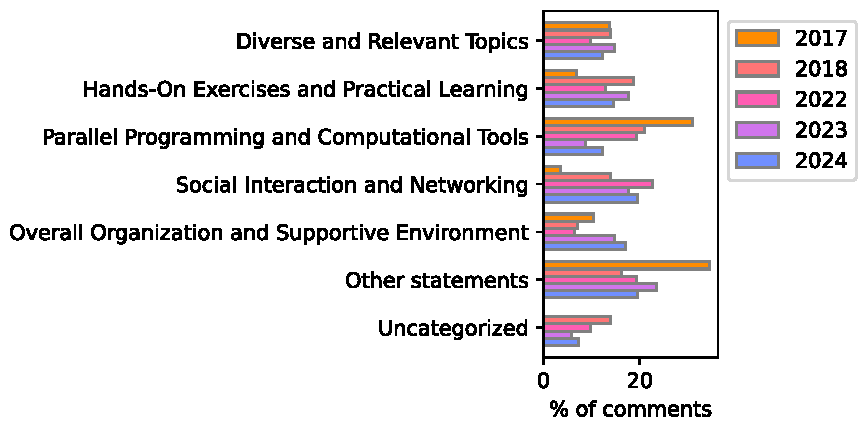
\includegraphics[height=4 cm]{PLOTS/like_most_categorization.pdf}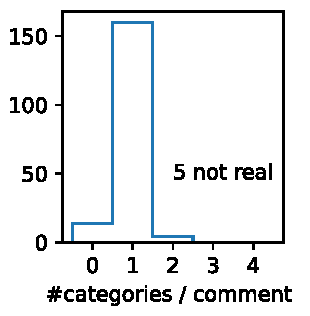
\includegraphics[height=3 cm]{PLOTS/like_most_categorization_hist.pdf} \hfill \mbox{ }
\end{minipage}
\end{tcolorbox}
\end{uncoverenv}
\end{frame}

\begin{frame}{``What did you like least about the school?''}
\tiny
\vspace{0.25 cm}
\begin{columns}
\column{1.1\linewidth}
{\bf\small Machine Learning and Lecture Pace}

Many students expressed concerns about the pace and structure of the machine learning sessions. The lectures were often described as rushed, chaotic, or difficult to follow, with insufficient time for hands-on exercises or deeper understanding of the material. There was a desire for more structured, interactive sessions and a broader introduction to machine learning concepts. Some students also felt that certain lectures moved too quickly over material, making it hard to grasp the content effectively.

\vspace{0.2 cm}
{\bf\small Living Conditions and Accommodations}

A significant number of participants were dissatisfied with the dormitory conditions, including the cleanliness and comfort of the rooms and bathrooms. Issues with bedding, humidity, and pests were mentioned, as well as discomfort with shared facilities. Some students felt the living arrangements detracted from their overall experience at the school.

\vspace{0.2 cm}
{\bf\small Time Constraints and Schedule}

The schedule of the school was a common concern, with many students feeling that the days were too packed, leaving insufficient time for rest, understanding, and application of the material. Early morning starts and long, intensive days contributed to fatigue and limited the ability to fully engage with the content. A longer duration for the school was suggested to allow more time for exercises and in-depth exploration of topics.

\vspace{0.2 cm}
{\bf\small Technical and Organizational Issues}

Several students experienced technical difficulties during the sessions, which affected their learning experience. Problems with software setup, internet connectivity, and technical support were noted. Some lectures were poorly organized, with inconsistent setups for exercises and technical issues that interrupted the flow of learning. There was a call for better preparation and organization to streamline these processes.

\vspace{0.2 cm}
{\bf\small Content Relevance and Diversity}

Some students felt that the content of the school was too focused on specific areas, such as the Large Hadron Collider (LHC), and did not cater to a broader range of interests within high energy physics. There were also comments on the lack of diversity among presenters and topics, and a desire for more inclusive and varied subject matter that would appeal to a wider audience.

\vspace{0.2 cm}
{\bf\small Other statements}

Some students had generally positive experiences and did not express specific complaints about the school. There were comments about the physical environment, such as classroom temperature and weather, as well as minor logistical issues like timing of start times. A few remarks pointed to specific lectures or speakers that did not meet expectations, either due to presentation style or content relevance. Overall, the feedback included a mix of satisfaction and minor grievances not directly related to the main categories identified.

\end{columns}

\begin{uncoverenv}<2->
\vspace{-5 cm}
\begin{tcolorbox}[colback=white, colframe=black]
\begin{minipage}{\linewidth}
\mbox{ } \hfill 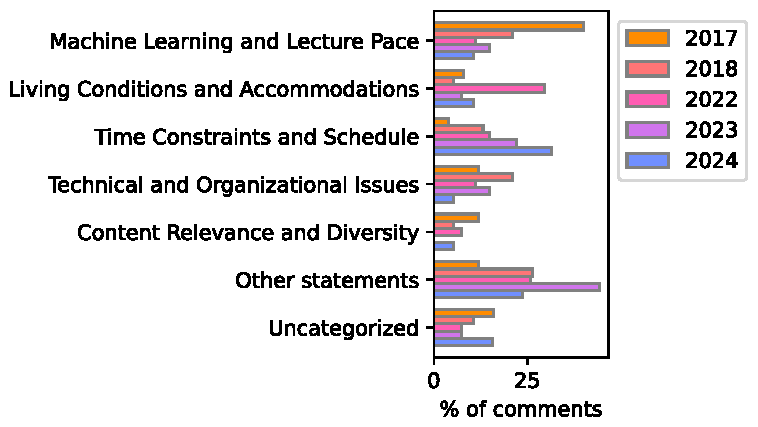
\includegraphics[height=4 cm]{PLOTS/like_least_categorization.pdf}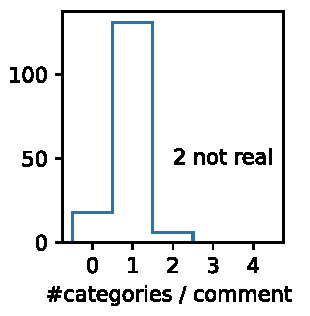
\includegraphics[height=3 cm]{PLOTS/like_least_categorization_hist.pdf} \hfill \mbox{ }
\end{minipage}
\end{tcolorbox}
\end{uncoverenv}
\end{frame}

\begin{frame}{``Any other general comments, feedback, or suggestions?''}
\tiny
\vspace{0.45 cm}
\begin{columns}
\column{1.1\linewidth}
{\bf\small General Appreciation and Positive Feedback}

\vspace{0.1 cm}
Participants consistently expressed gratitude and positive feedback about the school. Many found the experience enlightening, well-organized, and beneficial for their academic and professional growth. The workshops and lectures were generally well-received, with attendees appreciating the opportunity to learn and network with peers and experts in the field.

\vspace{0.2 cm}
{\bf\small Suggestions for Program Improvement}

\vspace{0.1 cm}
Participants suggested that the program could be improved by extending its duration, providing more time for hands-on exercises, and offering parallel sessions to cater to different levels of expertise in topics like machine learning. Some attendees recommended adding competitions, extra challenges, or large projects to foster engagement and practical application of skills learned.

\vspace{0.2 cm}
{\bf\small Logistical and Organizational Concerns}

\vspace{0.1 cm}
Several participants noted logistical issues, such as the need for clearer setup instructions before the event, better coordination with support staff, and improvements to room conditions. Suggestions included pre-event setup instructions, solutions for technical difficulties, and improvements to venue facilities to enhance the learning experience.

\vspace{0.2 cm}
{\bf\small Diversity and Inclusivity Concerns}

\vspace{0.1 cm}
There were concerns raised about diversity and inclusivity, particularly regarding gender and racial representation among participants and presenters. Suggestions included incorporating diversity statements and being mindful of inclusivity during all school activities to ensure a comfortable environment for everyone.

\vspace{0.2 cm}
{\bf\small Food and Accommodation Feedback}

\vspace{0.1 cm}
Feedback on food and accommodation was mixed, with many praising the quality and variety, while others suggested improvements such as offering vegan or halal options and addressing environmental concerns about waste. These aspects significantly influenced the overall satisfaction of participants during the school.

\vspace{0.2 cm}
{\bf\small Other statements}

\vspace{0.1 cm}
Some participants expressed gratitude and shared additional logistical suggestions, such as providing a clearer schedule, enhancing communication, and organizing campus tours. There were also comments on the importance of providing a welcoming and inclusive environment, even in informal settings like meals and social events.

\end{columns}

\begin{uncoverenv}<2->
\vspace{-5 cm}
\begin{tcolorbox}[colback=white, colframe=black]
\begin{minipage}{\linewidth}
\mbox{ } \hfill 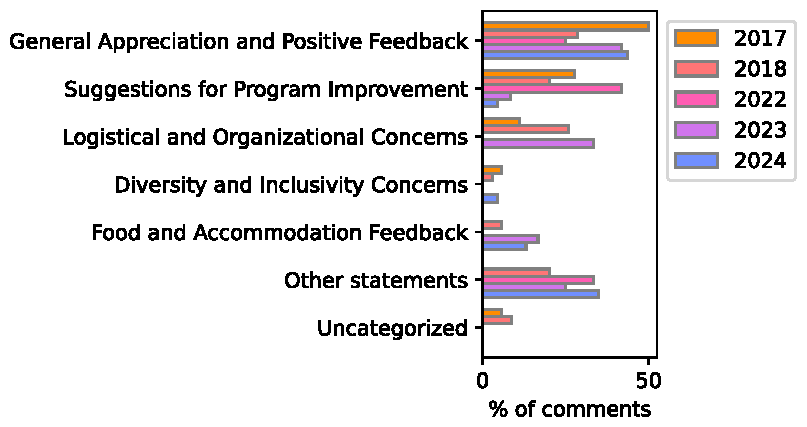
\includegraphics[height=4 cm]{PLOTS/general_feedback_categorization.pdf}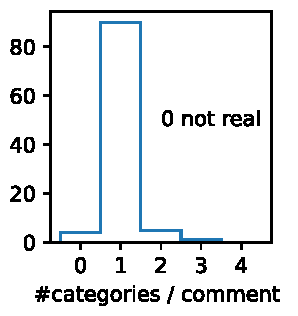
\includegraphics[height=3 cm]{PLOTS/general_feedback_categorization_hist.pdf} \hfill \mbox{ }
\end{minipage}
\end{tcolorbox}
\end{uncoverenv}
\end{frame}

\begin{frame}{``Should we extend the school to two weeks?'' (2024 only)}
\tiny
\vspace{0.45 cm}
\begin{columns}
\column{1.1\linewidth}
{\bf\small Concerns About Length and Format}

\vspace{0.1 cm}
Some participants express concerns about extending the school to two weeks. They believe that a longer duration might make it difficult for students to attend due to commitments at their home institutions. Suggestions include keeping the school format similar to a course that offers credits, making the program flexible, or maintaining a shorter duration like a week. Moreover, improvements in accommodations and facilities are considered necessary if the school is extended, as well as structured social programming to balance the intensive schedule.

\vspace{0.4 cm}
{\bf\small Benefits of Extended Duration}

\vspace{0.1 cm}
Extending the school to 10 days or two weeks is seen as an opportunity to delve deeper into the topics. Participants suggest more time for exercises, hands-on work, and small group projects. A longer duration could also allow for covering more material or exploring specific topics in greater depth, such as machine learning or neural networks. This could enhance the overall learning experience by providing students with more time to digest and apply the knowledge.

\vspace{0.4 cm}
{\bf\small Suggestions for Structure and Content}

\vspace{0.1 cm}
Participants recommend structuring the school to include shorter days, more free time, and breaks to prevent burnout. Incorporating group projects and social activities can enhance interactions among students. Suggestions include starting later in the day, including local cultural activities, and allowing time for students to explore independently. There is also a proposal to extend the school incrementally and gather feedback each year to refine the experience.

\vspace{0.4 cm}
{\bf\small Other statements}

\vspace{0.1 cm}
Some participants express general support for extending the school without specific suggestions for improvements. Others feel the current duration suffices for the material covered, while one participant expresses enthusiasm but acknowledges potential challenges in attending a longer program.
\end{columns}

\begin{uncoverenv}<2->
\vspace{-5 cm}
\begin{tcolorbox}[colback=white, colframe=black]
\begin{minipage}{\linewidth}
\mbox{ } \hfill 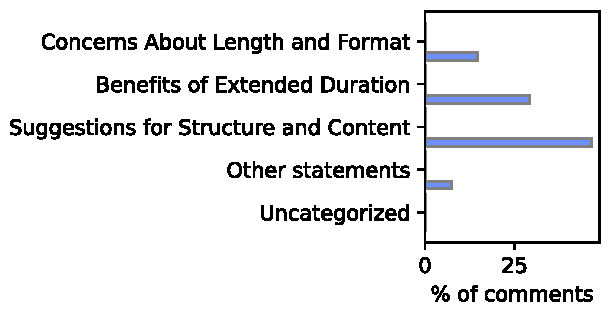
\includegraphics[height=4 cm]{PLOTS/two_weeks_categorization.pdf}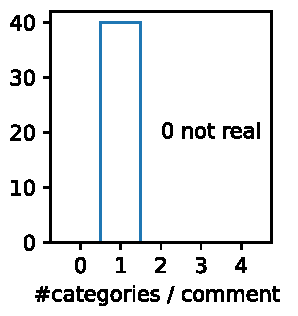
\includegraphics[height=3 cm]{PLOTS/two_weeks_categorization_hist.pdf} \hfill \mbox{ }
\end{minipage}
\end{tcolorbox}
\end{uncoverenv}
\end{frame}

\begin{frame}{Conclusions from student surveys}
\vspace{0.5 cm}
\large
\begin{itemize}\setlength{\itemsep}{0.5 cm}
\item<1-> Hands-on exercises are highlighted as important.
\item<2-> The topics are about right, but the applications are a little too LHC-focused.
\item<3-> We've had problems (and high turn-over) with the machine learning content, but it's decreasing.
\item<4-> New ideas: pre-event preparatory content and/or parallel sessions.
\item<5-> Students enjoy the in-person aspect of the school, though not the accommodations, and are split on whether it should be extended to two weeks. Those in favor want a longer, lower-intensity event; those opposed think that a longer school would conflict with other obligations.
\end{itemize}
\end{frame}

\end{document}
